\chapter{Detecting Twitter events}


\section{Introduction}
Twitter has been used to detect or predict a large variety of events,
from flood prevention \cite{de2017towards} to stock market movements
\cite{pagolu2016sentiment}. However, the specificity of social network data (short texts, use of
slang, abbreviations, hashtags, images and videos, very
high volume of data) makes all "general" detection tasks
(without specification
of the type of topic)
very difficult on tweet datasets.

Many works on event detection are actually
focused on burst detection (detecting topics such as
natural disasters, attacks, etc., that cause an unusual
volume of tweets), and do not attempt to assess the
relative size of events. We seek to detect \textit{all} events, both
those that generate a high volume of tweets and those that
are little discussed, and to group together \textit{all} tweets
related to the same event. With this definition in mind, the
topic detection and tracking task is conceptually similar to 
clustering. Given the size of our tweet collection, 
the chosen clustering method has to be extremely time-efficient.

Apart from the choice of the event detection algorithm, 
we also have to consider the type of tweet representation: 
should we only use the text of the tweets, or should we consider 
the tweet as a multimodal document, composed of text and/or images, videos, hashtags?

In the field of language processing, recent works
have made it possible to reach performance close to human capacity
in several tasks, 
particularly with regard to the evaluation of the semantic similarity 
between two sentences\footnote{See the results on the GLUE benchmark: \url{https://gluebenchmark.com/leaderboard}}. However, these advances, 
based on the training of neural networks on very large corpora of texts,
may not always be suited to our task. Indeed, despite rapid progress 
in recent years in the adaptability of
language processing (the GLUE benchmark \cite{wang2018glue} consists of
9 different tasks, and the models are evaluated according to their average performance on
all these tasks), it remains difficult to adapt these models to new tasks. 
Any transformation of the initial task requires fine-tuning a neural network 
on (at least) a few thousand sentences, which
involves hours of manual annotation to create a suitable dataset. 
In our work we focus on short-text topic similarity (evaluate if two sentences / short texts
address the same subject), which in some cases differs from semantic similarity
(evaluate whether two sentences mean the same thing) evaluated in GLUE, and we don't 
have a corresponding training dataset. Besides, even on a strictly identical
task, the performances announced in the litterature are perfectly reproducible 
only on English language corpora. 

Finally, most of these models are designed to be used as input to
end-to-end systems. For example, to calculate a similarity score between sentences
with BERT \cite{devlin2018bert}, it is necessary to treat each couple of sentences instead of each sentence. Using the example proposed in \cite{reimers_2019_sentence}, to find the two most similar sentences in a corpus of $n = 10,000$ sentences, the number of treatments to be performed is $n\frac{(n - 1)}{2} = 49,995,000$ operations, which represents approximately 65 hours of processing with BERT on a V100 GPU.
These architectures do not apply well to information retrieval systems that involve comparing
hundreds of thousands of sentences. For clustering or information retrieval tasks, 
it is more efficient to represent each sentence in a vector space where similar sentences
 are close (so-called \textit{embeddings}), and then apply conventional distance measurements 
 (cosine, euclidean distance, etc.).
 
 \begin{figure*}
  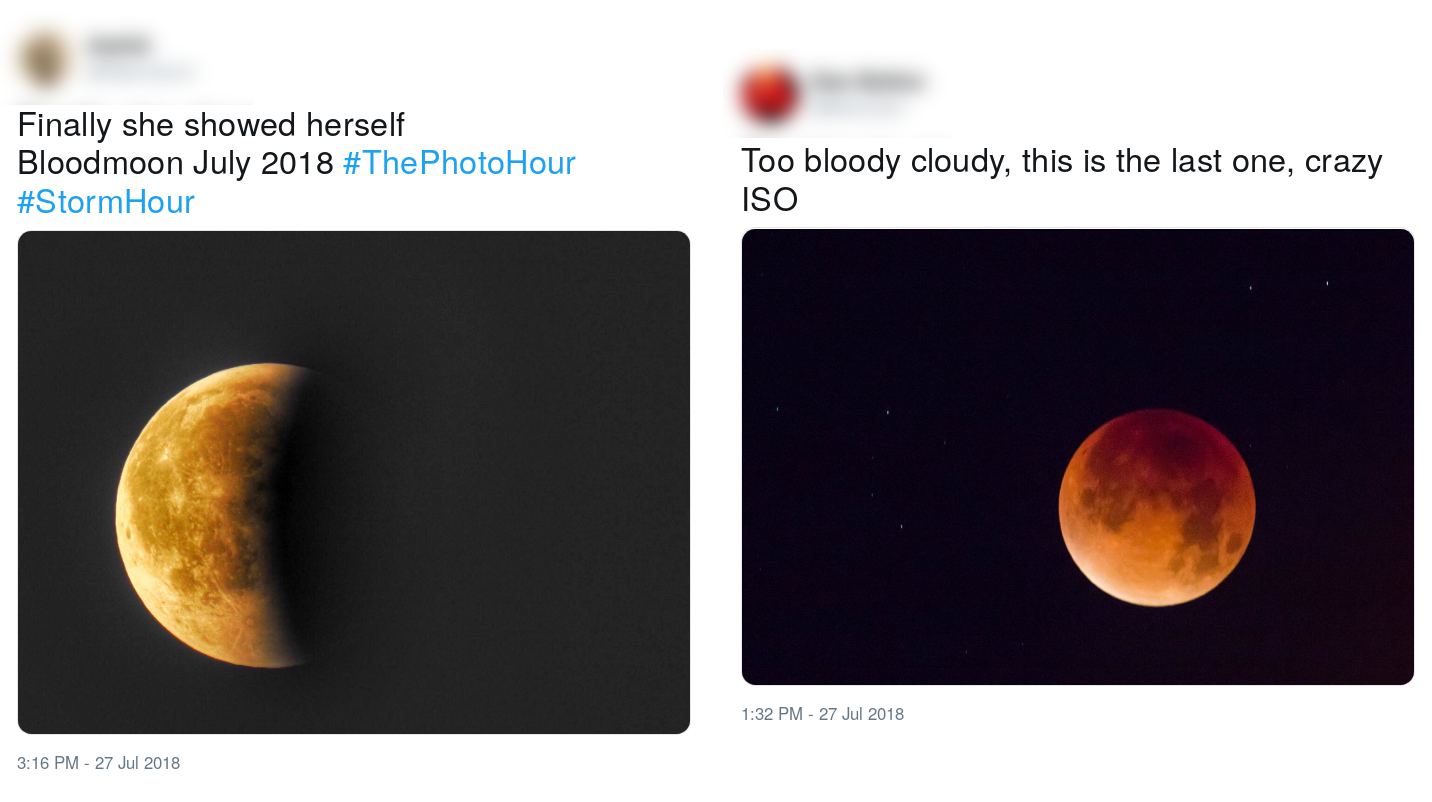
\includegraphics[width=\textwidth]{figures/Moon_horizontal.png}
    \caption{Example of a topic (the July 2018 lunar eclipse) where multimedia contents provide a critical information for topic detection}
    \label{fig:moon}
\end{figure*}
 
 Regarding images, recent progress in the field of visual content description due to deep neural networks provides new ways of representing social media documents by including rich visual features. There are cases where image provides decisive information for event detection (see Fig. \ref{fig:moon}). However, dealing with image tweets often requires a contextual knowledge external to the document. Without this knowledge, image can become a source of error for event detection algorithms compared to text alone.
 
 In this chapter, we show that the First Story Detection clustering algorithm is the most suitable for our event detection task. We show that the best vector representation of tweets for the FSD algorithm is the tf-idf approach. We compare this algorithm with another standard algorithm (DBSCAN) and a method from the literature (pDMM). We are also testing a two-step clustering method, to group tweets according to their textual content and then according to their visual content.
 
We conduct our demonstration by starting with a review of the state of the art, then a presentation of the different algorithms tested, before detailing the different text and image embeddings used as inputs to the FSD and re-clustering algorithms. Finally, we present our results in detail.


\section{State of the art}

		
		\subsection{Twitter event detection approaches}
		We divide the event detection methods into three types of approaches: term-weighting-based approaches, topic modeling, and clustering. This is also the classification used in the survey on real-time event detection by \citet{hasan_survey_2018}. The last approach, clustering, is dealt with in more detail in this state of the art, as it is the one we chose to implement for our own event detection tool.
		
		\subsubsection{Term-weighting-based approaches}
		These approaches rely on tracking the terms likely to be linked to an event (often due to a high frequency of some terms during a given time window). They usually return a list of the top $k$ trending events on Twitter, which does not meet our objective of detecting events in an exhaustive manner.
		
		The event detection system TwitterMonitor \citep{mathioudakis_twittermonitor:_2010} detects bursty keywords in the Twitter stream by comparing their term frequencies in previous periods to current term frequency. Bursty keywords are then grouped together in ``trends" depending on their co-occurrences in recent tweets. 
		
		EnBlogue \citep{alvanaki_see_2012} measures the correlation of hashtags pairs within a given time window. Emergent topics are then detected among the pairs with the highest shift in their correlation. EnBlogue produces an overall scoring of the topics depending on the shift in correlation and on the total popularity of each topic. This score is smoothed in order to give a higher rank to new topics. 
		
		MABED \citep{guille_event_2015} does not only use the textual content of the tweets: the frequency at which users interact with each other using ``mentions" (i.e. the name of another Twitter account preceded by ``@") is also taken into account to detect events. The system models the number of tweets that contain word $t$ and at least one mention during a given time-window as a binomial distribution. It detects positive anomalies if the creation of mentions associated to word $t$ is strictly greater than the expectation of the model. The magnitude of impact of an event on a time interval I is computed by integrating the anomaly function on the interval I. For each word associated with a mention, the system finds the interval I that maximizes its magnitude of impact. After other steps of event description and duplicates removal, the events with the highest impact are returned.
		
		The Twitter Live Detection Framework (TLDF) \citep{gaglio_framework_2016} modifies the Soft Frequent Pattern Mining (SFPM) algorithm \citep{petkos_soft_2014} to adapt to the dynamic nature of tweets. The authors use the relevance score of term $t$ proposed for SFPM: the ratio of the likelihood of appearance of the term in the current time-window and in a reference set of tweets. This relevance score is combined with a parameter boosting the score of named entities and multiplied by the $\mbox{tf-idf}$ of term $t$. Moreover, the size of the detection time-window is not fixed, but is controlled by a sigmoid function depending on the volume of emitted tweets at a given moment.
	
	\subsubsection{Topic models} 
	\label{topic models}
	Topic models are widely used techniques in the natural language processing field to discover the topical structure from a corpus of textual documents (news articles, scientific papers, tweets, etc.). Latent Dirichlet Allocation (LDA) is the most common one \citep{blei_latent_2003}. In this model, each document is considered as a mixture of different topics drawn from a topic distribution. In the case of topic detection in a collection of tweets, LDA has several drawbacks: 1.the model does not take into account the fact that topics change over time 2. the number of topics has to be known in advance 3. it assumes that a document is a mixture of several topics, which is very rare in short texts like tweets. There is however a vast literature working on strategies to overcome these limitations.
	
	Concerning the first point, \citet{blei_dynamic_2006} have addressed the issue of topics evolving over time; however they assume that the number of topics remains the same over periods, whereas in a stream of tweets, topics can emerge and disappear at each new period.
	
	Regarding the number of topics, some methods exist to estimate the optimal parameter $k$  \citep{brunet_metagenes_2004,arun_finding_2010,greene_how_2014}. However these methods rely on re-generating topic models for each candidate $k \in [k_{min}, k_{max}]$. This can be achieved for a small number of topics ($k_{max} < 100$), but testing each $k$ in a range $[2100, 10500]$ (between 100 and 500 events a day in our corpus of 21 days) is not an option. 
	
	Regarding the third assumption, a number of articles have specifically tackled the issue of applying topic models to short texts. The recent survey by \citet{likhitha975detailed} summarizes the topic modeling techniques used to find topics within short text documents.
    
    Based on the assumption made by \citet{nigam2000text} that each document is assumed to be generated from a single topic, that is, the words within a document are all sampled from the same topic distribution, \citet{yin_dirichlet_2014} propose the Dirichlet Multinomial Mixture (DMM) model. The generative process of DMM can be described as follows: 
    \begin{center}
        	\begin{enumerate}
	 	\item Choose a proportion of topics $\theta \sim Dirichlet(\alpha)$.
	 	\item For each topic $k \in \lbrace1,\ldots,K\rbrace$:
	 	 
			Draw a distribution of words linked to this topic $\phi_k \sim Dirichlet(\beta)$.
		\item For each document $d \in \lbrace1,\ldots,D\rbrace$:
		\begin{enumerate}
		    \item Draw a topic $z_d \sim Multinomial(\theta)$.
		    \item For each word $w$:
		    
		    Draw a word $w \sim Multinomial(\phi_{z_d})$
		    
		\end{enumerate}	 	  
	 \end{enumerate}
    \end{center}

\citet{yin_dirichlet_2014} provide a collapsed Gibbs Sampling algorithm (GSDMM) to approximate the hidden variables in this generative process. The interest of this method in our case is that over iterations, some clusters (topics) become empty, while others progressively gather more documents. This means that the algorithm can approximate the number of documents in the collection, as long as the initial number of topics (K) is large enough at initialization. DMM is therefore very relevant to our study because it addresses both problem 2. (number of clusters unknown) and problem 3. (only one topic per tweet).

This simple and efficient method has been adapted and improved by several authors:
\citet{nguyen2015improving} integrates Word2Vec embeddings into DMM by replacing the topic-word Dirichlet multinomial component with a draw from a Bernoulli distribution to determine whether the Dirichlet multinomial component or a word embedding component will be used to draw the word $w$. \citet{li_enhancing_2017} propose PDMM, an extension of the DMM model by allowing short texts to be generated from one to three topics and drawn from a Poisson distribution, and GPU-PDMM, that exploit word-embeddings to enrich the latent topic learning with external semantic relations. 

However, these advances seem to increase calculation times by several orders of magnitude. \citet{li_enhancing_2017} provide a comparative table of the time efficiency of these different models, which we compare with their accuracy in Table \ref{Tab: BenchmarkDMM}. According to their experiments (all models are implemented in Java), the extended DMM models seem to multiply by 10 or even 100 the calculation time of plain DMM, on the BaiduQA dataset\footnote{a corpus of 648,514 questions from a Chinese Q\&A website, containing 35 labels.} for an increase in accuracy of 2 to 3 points. Therefore, we decided to use DMM as comparison model with the First Story Detection algorithm (see next Section) rather than more recent approaches.


%%%%%%%%%%%%%%%%%%%%%%%%%%%%%%%%%%%%%%%%%%%%%%%%%%%%%%%%%%%%%%%
\begin{figure}[h]
\centering
\begin{subfigure}{.5\textwidth}
  \centering
  \rowcolors{2}{white}{gray!25}
  \begin{tabular}{|l|ccc|}
\hline
\textbf{Model} & \textit{K=40} & \textit{K=60} & \textit{K=80} \\
\hline
           DMM &         0.355 &         0.566 &         0.843 \\
        LF-DMM &          13.0 &          20.5 &          31.8 \\
          PDMM &          11.6 &          11.7 &          11.8 \\
      GPU-PDMM &          37.8 &          40.7 &          45.2 \\
\hline
\end{tabular}

  \caption{Time cost (in seconds) per iteration of each model}
  \label{Tab: time_efficiency}
\end{subfigure}%
\begin{subfigure}{.5\textwidth}
  \centering
  \rowcolors{2}{white}{gray!25}
  \begin{tabular}{|l|ccc|}
\hline
\textbf{Model} & \textit{K=40} & \textit{K=60} & \textit{K=80} \\
\hline
           DMM &         0.523 &         0.548 &         0.553 \\
        LF-DMM &         0.424 &         0.449 &         0.487 \\
          PDMM &         0.553 &         0.562 &         0.577 \\
      GPU-PDMM &         0.545 &         0.569 &         0.583 \\
\hline
\end{tabular}

  \caption{Average classification accuracy of each model}
  \label{Tab: classification_accuracy}
\end{subfigure}
\caption{Comparison of time efficiency and classification accuracy of several DMM-adapted models with different numbers of topics $K$ on the BaiduQA dataset. These values are provided by \citet{li_enhancing_2017}}.
\label{Tab: BenchmarkDMM}
\end{figure}
%%%%%%%%%%%%%%%%%%%%%%%%%%%%%%%%%%%%%%%%%%%%%%%%%%%%%%%%%%%%%%
 	 


	\subsubsection{Dynamic clustering \label{Subsubsec: incremental clustering}} Dynamic clustering approaches do not require a fixed number of clusters. These methods are well fitted for discovering clusters of textual documents dynamically as new documents are added to the collection. For this type of clustering, the algorithms that are often used take into account both the thematic similarity of the documents and their temporal proximity, in order to avoid grouping in the same cluster tweets sent at very distant times. This type of approaches generally use the state-of-the-art First Story Detection (FSD) \citep{allan_introduction_2002} algorithm as a reference method. In this method (see Algorithm 1), documents are represented using tf-idf (see Section \ref{Text embeddings} for a presentation of tf-idf encoding), their similarity is computed using cosine similarity, and each new document joins the cluster of its nearest neighbor in the collection. If the distance to the nearest neighbor is higher than a pre-defined threshold $t$ a new cluster is created, that contains the new document. Regularly, the oldest documents are dropped from the collection. This insures that each new document is only compared to the most recent documents. 

%%%%%%%%%%%%%%%%%%%%%%%%%%%%%%%%%%%%%%%%%%%%%%%%%%%%%%%%%%%%
\begin{algorithm}
\caption{``First Story Detection"}
\begin{algorithmic}[1]
\REQUIRE threshold $t$, window size $w$, corpus $C$ of documents in chronological order
\ENSURE thread ids for each document
\STATE $T \leftarrow \left[ \right] ; i \leftarrow 0 $
\WHILE{document $d$ in $C$}
\IF{$T$ is empty}
\STATE $thread\_id(d) \leftarrow i$
\STATE $i \leftarrow i+1$
\ELSE
\STATE $d_{nearest} \leftarrow $ nearest neighbor of $d$ in $T$
\IF{$cosine(d, d_{nearest}) < t$}
\STATE $thread\_id(d) \leftarrow thread\_id(d_{nearest})$
\ELSE
\STATE $thread\_id(d) \leftarrow i$
\STATE $i \leftarrow i+1$
\ENDIF
\ENDIF
\IF{$|T| \geq w$}
\STATE remove first document from $T$
\ENDIF
\STATE add $d$ to $T$
\ENDWHILE
\end{algorithmic}
\end{algorithm}
%%%%%%%%%%%%%%%%%%%%%%%%%%%%%%%%%%%%%%%%%%%%%%%%%%%%%%%%%%%%



Existing works on tweet incremental clustering have adapted this reference method initially developed for streams of news (such as RSS streams) to process much higher volumes of documents, and very short texts. Indeed the maximum size of a tweet is 280 characters (140 characters before 2018). Changes in that baseline method are done either in the type of text representation, or in the clustering algorithm itself. A step of noise filtering is also frequently added before the clustering step, to distinguish event from non-event tweets (according to \citet{liu_reuters_2016}, the proportion of event tweets in well-established corpora such as the one by \citet{mcminn_building_2013} is less than 0.2\%). This section explores the variations introduced in the clustering algorithm.


In TwitterStand, \citet{sankaranarayanan_twitterstand:_2009} first perform a filtering step, that classify tweets as either ``junk" or ``news" using a naive Bayes classifier. Then, their online clustering algorithm associates a vector to each cluster, which is composed from the contained tweets' terms weighted with tf-idf. Each new tweet is represented using tf-idf and compared to the clusters' vectors using a modified cosine distance that accounts for the temporal dimension of clusters. The distance formula is 
$$
\dot{\delta}(t,c) = \delta(t,c)\times e^{\frac{-(T_t-T_c)^2}{2\sigma^2}}
$$

\noindent where $\delta(t,c)$ is the cosine distance between tweet $t$ and cluster $c$, $T_t$ is tweet $t$'s publication time and $T_c$ is cluster $c$'s mean publication time. The distance is only computed for clusters with a mean publication time $T_c$ more recent than 3 days, and that have a word in common with $t$. If $\dot{\delta}(t,c^*) \leqslant \epsilon$ (where $c^*$ is the nearest cluster to $t$), the tweet $t$ is added to the cluster $c^*$. Else, a new cluster is created. To speed up the search for the nearest cluster, an inverted index of the cluster's words is maintained: for each word $w$, the inverted index stores pointers to the clusters that contain $w$. The clustering algorithm in TwitterStand is adapted to the noisy nature of tweets by maintaining a list of reputable sources. A cluster is dropped from the list of active clusters if none of the first $k$ tweets are from a reputable source. The system also deals with fragmentation (the fact that several clusters about the same topic are created) by removing duplicate clusters. If a cluster $c'$  is identified as the duplicate of an older cluster $c$, $c'$ is marked as ``slave" of the cluster $c$, and $c$ as ``master" of $c'$. Any tweet that should be added to $c'$ is now added to $c$.

\citet{petrovic_streaming_2010} speed up the standard FSD algorithm by replacing the nearest neighbor search by an approximate nearest neighbor search using Locality Sensitive Hashing. Instead of searching for the nearest neighbor in the set of all documents, the search is done among a small set $S$ of potential nearest neighbors. The set $S$ is the set of documents that have the same hash as current document $x$:
$$
S(x) = \{y: h_{ij}(y) = h_{ij}(x), \exists i \in [1 \ldots L], \forall j \in [1 \ldots k]\}
$$
where $L$ is the number of hash tables, and $k$ the number of hyperplanes in each hash table. The hash functions $h_{ij}$ are defined as:
$$
h_{ij}(x) = sgn(u_{ij}^Tx)
$$
the sign of the scalar product of random vector $u_{ij}$ and $x$. To reduce the risk of failing to find the nearest neighbor (if the nearest neighbor $y$ does not collide with $x$ in the set $S(x)$), if no nearest neighbor is found, the system starts a search of exact nearest neighbor through an inverted index containing only most recent documents. To limit the growth of the sets $S$ (also called buckets), the number of documents in a single bucket is limited to a constant parameter. The oldest documents in the bucket are then removed. 

The system proposed by \citet{petrovic_streaming_2010} has later been improved by the same authors \citep{petrovic_using_2012} using public synonym and paraphrase corpora in order to expand the words of the tweets with all their potential synonyms. This approach is a way to compensate for the scarcity of information contained in tweets and to increase the chances of finding a potential neighbor even if there is no tweet containing the same words in the collection.

\citet{becker_beyond_2011} use the same clustering algorithm as \citet{sankaranarayanan_twitterstand:_2009}, with each new tweet being represented as a tf-idf vector and compared using cosine similarity to the centroid of each cluster (the centroid is the mean weight of all terms in all tweets contained in the cluster). The specificity of their approach lies in the step following the clustering: instead of processing to a noise/event classification at the tweet level, the classification step takes place at the cluster level. They use a wide range of features in order to run a classification algorithm able to distinguish event clusters from noise clusters. The considered features are temporal features (taking into account the frequency of emission of the tweets in the cluster), social features (percentage of messages being retweets, replies, or mentions), topical features (based on the assumption that event clusters have a smaller diversity of topics), and Twitter-Centric features (hashtag usage, presence of multi-word hashtags).

\citet{mcminn_real_2015} base their event-detection approach on Part Of Speech (POS) Tagging and Named Entity Recognition (NER). Their first step is to extract named entities (persons, locations and organizations) and lemmatized nouns and verbs from each tweets. They then proceed to an aggressive filtering step (95\% of the tweets are removed): the system removes retweets, tweets with no named entities, and tweets containing terms associated with noise (``follow", ``watch", etc.). Then two steps are conducted in parallel: a clustering and a burst detection step. The clustering is based on an inverted index of all named entities: for each new tweet, the tweets containing the same named entities are retrieved from the index. The nearest neighbor is searched among these tweets using tf-idf representation, cosine similarity and a similarity threshold. If a nearest neighbor is found and does not already belong to a cluster, a new cluster is created containing the two tweets. In parallel, the burst detection module looks for bursts in the frequency of the detected entities. Once a burst has been detected, the clusters associated with the given entity are associated to it if the average timestamp of the tweets in the cluster is after the initial burst. The clusters associated to one burst form an event. If an entity associated to another event is mentioned in more than 50\% of the event's tweets, the two events are merged.

With Reuters Tracer, \citet{liu_reuters_2016} propose an event detection system that is also largely based on POS tagging and NER. This system combines a tweet-level noise filtering and a cluster-level noise filtering. Are considered as ``noise" all tweets and all clusters of tweets that are not linked to an event (in the sense of \citet{mcminn_building_2013}). The clustering algorithm itself is quite different from the standard FSD algorithm. New tweets are added to clusters based on three criteria: (1) Retweets of the same tweets are all added to the same cluster. (2) Tweets containing the same url are all added to the same cluster. (3) Finally, a similarity metric with the existing clusters is computed as follows:
$$
S_i = aN_e + bN_n + cN_v + dN_h
$$
where $N_e,N_n,N_v,N_h$ are the numbers of matching Named Entities, nouns, verbs and hashtags between the tweet and the cluster, and $a, b, c, d$ are learned parameters. Liu and al. explain that their system is primarily based on named entities (``An event is usually defined by \textit{who}, \textit{where} and \textit{what}" according to \citet{mcminn_building_2013}), and that there is no need for high dimensional tf-idf vectors to compute a good similarity function. The obtained clusters, called ``unit clusters" are progressively merged into bigger clusters using the same steps (merging based on retweets, urls, then similarity metric) as the unit clustering step. However, the used $a, b, c, d$ parameters are different.

\citet{hasan_twitternews_2016} use the technique of First Story Detection with LSH developed by \citet{petrovic_streaming_2010}. However, they observe that the $k$ independent random vectors in a single hash table need to be updated every time the size of the input tf-idf vectors increases (which happens at a high rate in Twitter data since the vocabulary evolves faster than in traditional news media). To alleviate this problem, they propose a technique using random indexing \citep{sahlgren_introduction_2005}. Random indexing  aims at representing terms with fixed-size vectors. Each term $t$ is associated with two vectors: an index vector and a context vector. The index vector is a random vector. The context vector has the same size as the index vector and it is initialized with zeroes. When a co-occurrence of the term $t$ with another term $t'$ is observed, the context vector of $t$ is updated by adding the index vector of $t'$. A tweet can then be represented as an average of the vectors of each term in the tweet. This tweet representation is then used to perform the LSH approximate neighbors search of the tweet $d$. However, once the set $S$ of all documents that collide with $d$ in a hash table is computed, the exact nearest neighbor search is done using cosine similarity on tf-idf vectors, rather than random indexing vectors. \citet{hasan_twitternews_2016} use this method as a first algorithm in order to detect ``non unique" tweets, that are then clustered using a second algorithm close to the one by \citet{sankaranarayanan_twitterstand:_2009}: this time, the similarity to the clusters' centroids is computed. Hasan et al. explain the use of this two-steps clustering method by the necessity to restrain the number of ``one tweet clusters". A defragmentation step is finally done in order to merge similar clusters.


In these works, tweets are represented in the form of tf-idf vectors in the vast majority of cases \citep{sankaranarayanan_twitterstand:_2009, petrovic_streaming_2010, becker_automatic_2011, hasan_twitternews_2016}. \citet{repp_extracting_2018} test different types of representation of tweets (Word2Vec average, GloVe average, Doc2Vec, Word2Vec average weighted by the idf of each word). However, these representations are only tested on a classification task, and the best representation (the average of Word2Vec) is then used for clustering. We therefore wanted to update this work by testing recent embeddings, and in particular those developed for representation of sentences. The next section details recent advances in text embeddings, from word embeddings to sentence or short-text embeddings.

\subsection{Text embeddings}
\label{Text embeddings}
The most commonly used "vectorization" method until the 2010s
was the tf-idf, introduced by \citet{sparck_1972_statistical}. This is an improvement to the principle “bag of words” vectors \cite{harris1954distributional}, where each document is described by the
number of occurrences of the words it contains ("term frequency"). The tf-idf representation uses the same vectors, but weights each of the words in inverse proportion of the number of documents in which it appears.

\subsubsection{Word embeddings}

The publication of Word2Vec \citep{mikolov_efficient_2013} and GloVe \citep{pennington2014glove}, two methods based on the prediction of the context of each word (or the prediction of each word depending on its context), made it possible to create word vectors carrying semantics other than the word frequency in the corpus. However, these representations lost the ability to describe each document by a single vector. To get around this problem, each document is often represented by an average of word vectors.

With ELMo \citep{peters2018deep} appears a new generation of models,
allowing words to be represented not only depending on their usual context (the words with which they are frequently used in the training corpus), but also according to their local context: the word representation is specific to a given sentence. This constitutes an important advance in language processing, since a word no longer has a single representation that aggregates its different meanings, but several representations for each of the contexts in which it is used. ELMo is based on a bi-directional LSTM neural network trained to predict the next word in a sequence in both directions (i.e. predict the next word in a sentence, but also, given the end of a sentence, predict the word just before it). However, ELMo is not designed to produce sentence embeddings, but to be used as input to task-specific neural models. Nevertheless, the authors test the performance of word vectors directly from the first or second layer of their model (which contains three layers) for a disambiguation task by searching for the first nearest neighbor. The results obtained are close to the state of the art.

BERT \cite{devlin2018bert} is even more generic than ELMo, because this model does not require a specific architecture for each type of task: it can be fine-tuned to a new dataset by simply adding an output layer. BERT is built with a Transformer-type architecture \cite{vaswani2017attention}, and pre-trained on two types of tasks: predicting hidden words in a sentence and predicting the next sentence in a text. As in ELMo, the authors of BERT do not intend to create sentence embeddings from their model, but rather to provide an architecture that should be trained differently for each specific task. However, they demonstrate that a simple transfer learning (extraction of  word vectors used at the input of a new model without fine-tuning) can match the state of the art for a named entities detection task.

\subsubsection{Sentence embeddings}
\label{embedding_phrases}
There is a large number of works that attempt to represent sentences by generic vectors that can be used in a wide variety of tasks, especially for transfer-learning. 
For example, Skip-Thought \citep{kiros2015skip} is based on an encoder-decoder architecture trained to generate the sentences framing a given sentence in a text.

\citet{conneau2017supervised} show with InferSent, a bi-directional Siamese LSTM network (Siamese means that it takes two sentences as input, but applies the same weights in both parts of the network), that supervised learning provides better results for the creation of generic sentence vectors. InferSent is trained on a classification task using the SNLI dataset \cite{bowman2015large}, which contains $570,000$ pairs of English sentences manually annotated in three categories: the first sentence implies the second, the first sentence contradicts the second, or the first sentence and the second sentence are mutually neutral.

With Universal Sentence Encoder, \citet{cer2018universal} apply the results of \citet{kiros2015skip} and \citet{conneau2017supervised} by training a Transformer architecture both on unsupervised tasks, as it was done for Skip-Thought, and on the SNLI dataset, like InferSent. 

Sentence-BERT \cite{reimers_2019_sentence} does not provide universal vectors, but a fine-tuning architecture of the BERT model specifically adapted to produce sentence embeddings adapted to certain types of tasks. This model modifies BERT into a Siamese network, with a final layer depending on the type of task on which the network is trained. The authors test their representations on the STS dataset \cite{cer2017semeval} ($8,628$ pairs of sentences with a similarity score between 0 and 5) by computing a simple cosine similarity score between the vectors associated with each sentence. They show that the best performances on the STS dataset are obtained by a first fine-tuning on SNLI and then a second fine-tuning on the STS training set.

All these embedding methods are potential ways of representing the text of tweets. We compare their performance in Section \ref{Subsec: text embeddings}. However, we were also interested in the information carried by the image, because communication on social networks is increasingly carried by visual supports. The next section reviews the existing literature on multimodal event detection.

\subsection{Text-Image event detection}

In the last three years, some works on Twitter data have started to use multimodal embeddings to solve various tasks: \citet{lu2018visual} incorporate tweets pictures in order to improve Named Entities Recognition in the text of the tweets. Other works combine text and image of tweets in order to recommend hashtags \citep{zhang2017hashtag} or users mentions \citep{ma2018mention}. These approaches show that using visual and textual context for tweets-related tasks improves performance in several cases. Yet, it is unsure whether current visual content description systems can improve Twitter event detection. 


We found relatively little work on the joint use of image and text for the specific task of event detection in tweets. \citet{alqhtani2018multiple} use text and image to detect tweets related to earthquakes. They extract  visual features by using scale-invariant feature transform (SIFT) to
automatically detect keypoints from images. These keypoints are then clustered to generate a visual vocabulary. Images are then represented as "bags of visual words". Text is represented using tf-idf vectors. After a step of features selection using PCA, they use a linear combination of two kernels to train a classifier detecting "earthquake tweets" from other tweets. This contribution shows that a kernel fusion of text and image provides better results than text alone on the specific task of detecting earthquakes. However, these results do not give any conclusion on the role of the image in the detection of other types of events.

\citet{zhang2018novel} generate image captioning using an encoder-decoder neural architecture to enrich the text of tweets with a description of images. They then apply an improved-LDA algorihm to extract topics. The authors obtain better results with their method than with the tested "text-only" LDA approach. However, the evaluation corpus is rather small (only 10 subjects), and the selected topics favour the contribution of image, as they are subjects for which image captioning tools provide satisfactory results, such as "Giraffe", "Polar Bear" or "Sunrise".  

%%%%%%%%%%%%%%%%%%%%%%%%
\begin{figure}
\begin{center}

\includegraphics[width=1\textwidth]{figures/distracted_boyfriend.png}
\end{center}
{\scriptsize The two images present variations of the same meme, known as "Distracted Boyfriend". It is a classical example of meme, with identical visual content but different captions.
}
\caption{Example of a meme}
\label{Figure:meme}
\end{figure}
%%%%%%%%%%%%%%%%%%%%%%%%

The "MediaEval Social Event Detection" challenges \cite{reuter2013social, petkos2014social} have led to the publication of research articles on social event detection, unfortunately it is based on Flickr datasets. A description of the datasets is provided in Section \ref{state of the art}. Flickr is more an image hosting service than a social network: text plays a very limited role, and the images posted are personal photos rather than memes\footnote{A meme is an amusing image or video that is spread massively on the Internet, often with slight variations. See Figure \ref{Figure:meme} for a classical example of meme.} or images containing text.  

On Twitter, conversely, not all tweets contain images (in our annotated corpus, 23\% of tweets contain a visual
content - image, video or animated GIF.), and a very large part of the images contains text. \citet{chen2016context} find that 35\% of the images in their dataset contain text, mainly in the form of memes (37\%), photos of text (22\%) or tweet screenshots (8\%). Due to the high proportion of textual content and memes in Twitter images, the contribution of the image to the event detection task may be small or even negative compared to text alone, as tweets about very different events may contain the same image. In the remainder of this chapter, we test several types of text and image representations, as well as several types of event detection, in order to answer this question.

\section{Algorithms}

Different algorithms are tested in this chapter. In this section, we present them and explain how their parameters were tested. Some of these algorithms are not directly suited for our event detection task,
since they take the number of classes or topics as an input, whereas we need an algorithm capable of automatically discovering the optimal number of clusters. This is the case for SVM classifiers, that are rather used to evaluate the quality of different embeddings. In total, we present five methods: SVM classification, FSD algorithm, FSD algorithm with re-clustering, DBSCAN, and Dirichlet Multinomial Mixture model.

\subsection{Support Vector Machines (SVM)}
Evaluating the "quality" of tweet representations can be done according to different approaches: first, test if the representation allows a good separability of the different classes (events). Second, make sure that the vectors produced are suitable for distance measurements, which are used for clustering. To evaluate the separability of classes, we initially reduced the task of unsupervised event detection to a classification task. We used SVM classifiers with two types of kernel: a triangular kernel \cite{fleuret2003scale} and a Radial Basis Function (RBF) kernel. 

The triangular kernel function is the following:
\begin{align}
\label{eq:triangular kernel}
k(x, y) = 1 - \|x - y\|
\end{align}
Our experiments with this type of kernel show that, in addition to being invariant to scale changes \citep{fleuret2003scale}, it can be applied effectively to both dense and sparse vectors. It achieves performance similar to parametric kernels on text classification, with the advantage of not requiring a lengthy grid search process to select the right parameters.

Our first experiments were conducted only with a triangular kernel. However, as this is not a very well-known form, several reviewers have requested further tests to be conducted with a more common kernel. We therefore also conducted classification experiments with an RBF kernel:
\begin{align}
\label{eq:RBF kernel}
k(x, y) = \exp(-\gamma \|x - y \|^{2})
\end{align}
and performed a grid search to optimize the $\gamma$ parameter.

Both classifiers are trained on a random sample of 50\% of the corpus. The classification is evaluated by the macro average of the F1 score of each class.

\subsection{First Story Detection}
\label{Subsec: FSD}
 In a second step, we modelled the event detection problem more realistically as dynamic clustering, using a modified FSD algorithm. Our change consists in introducing "mini-batches" of tweets in order to parallelize the search for the nearest neighbor of each tweet in the batch. This modification may lower the performance of the algorithm, since the nearest neighbor of a given tweet may be in the same batch and therefore not found. In practice, with batches of 8 tweets, the probability that the nearest neighbor is in the same batch as the considered tweet is 0.15\% for our annotated French dataset.\footnote{The annotated French dataset contains 95,796 tweets on a period of 21 days. If we set the window parameter $w$ to one day of tweets (4562 tweets), the probability that the nearest neighbor of a given tweet is in the 8-tweets batch rather than in the rest of the window is $\frac{7}{4561}=0.0015$.}
 
 Our version of the algorithm also deals with "empty" documents, that is documents that contain no words or only stop-words. This is frequently the case in datasets of tweets. Empty documents are not clustered, \textit{i.e.} labeled as $-1$. Our version of the algorithm is described below:
 %%%%%%%%%%%%%%%%%%%%%%%%%%%%%%%%%%%%%%%%%%%%%%%%%%%%%%%%%%%%
\label{FSD}
\begin{algorithm}
\caption{``Mini Batch First Story Detection"}
\begin{algorithmic}[1]
\REQUIRE threshold $t$, window size $w$, batch size $b$, corpus $C=\{d_0 \ldots d_n\}$ of documents in chronological order
\ENSURE thread ids for each document
\STATE $T \leftarrow \left[ \right] ; i \leftarrow 0  ; j \leftarrow 0 $
\WHILE{$i < n$}
\STATE $batch = \{d_{i}, \ldots d_{i + b -1}\}$
    \FOR{document $d$ in $batch$}
    \IF{$d$ is empty}
    \STATE $thread\_id(d) \leftarrow -1$
    \ELSE
    \IF{$T$ is empty}
    \STATE $thread\_id(d) \leftarrow j$
    \STATE $j \leftarrow j+1$
    \ELSE
    \STATE $d_{nearest} \leftarrow $ nearest neighbor of $d$ in $T$
    \IF{$cosine(d, d_{nearest}) < t$}
    \STATE $thread\_id(d) \leftarrow thread\_id(d_{nearest})$
    \ELSE
    \STATE $thread\_id(d) \leftarrow j$
    \STATE $j \leftarrow j+1$
    \ENDIF
    \ENDIF
    \IF{$|T| \geq w$}
    \STATE remove first document from $T$
    \ENDIF
    \ENDIF
    \STATE add $d$ to $T$
    \STATE $i \leftarrow i + b$
    \ENDFOR
\ENDWHILE
\end{algorithmic}
\end{algorithm}
%%%%%%%%%%%%%%%%%%%%%%%%%%%%%%%%%%%%%%%%%%%%%%%%%%%%%%%%%%%%

The parameters of this algorithm are $w$ (number of past tweets among which we search for a nearest neighbor) and $t$, the distance threshold above which a tweet is considered sufficiently distant from past tweets to form a new cluster. The value of $w$ has been set differently for each corpus: it is set to approximately one day of tweets history, based on the average number of tweets per day in each corpus. We then tested different values of $t$ for each type of representation. Generally speaking, lower $t$ values lead to more frequent clustering, and thus better intra-cluster homogeneity (better precision), but may lead to over-clustering (lower recall).

Clustering performance is evaluated by a measure we call "best matching F1". It is defined by \citet{yang1998study}: we evaluate the F1 score of each pair between clusters (detected) and events (annotated). Each event is then matched to the cluster for which the F1 score is the best. Each event can be associated to only one cluster. The best matching F1 thus corresponds to the average of the F1s of the cluster/event pairs, once the matching is done.

We chose to use this metric, rather than the one defined by \citet{mcminn_real_2015}: they consider all clusters with more than 75 tweets as candidate events. A candidate is evaluated as true positive if 5\% or more than 15 tweets of the candidate's tweets match those of an annotated event. We denote $a$ the number of true positives. From the detail of their experimental results, we can deduce that all candidates that match with a ground truth's event are counted as true positives, even if several clusters match the same event. Conversely, all candidates that do not match an event from the ground truth are considered false positives. 

We decided not to use this metric for two reasons: first, we only have access to the portion of the \citet{mcminn_building_2013} dataset that was not deleted over time. Therefore, we cannot keep the threshold of 75 tweets per event, and we would not be able to compare our results with those obtained by McMinn and Jose. Second, this measure favors over-clustering by not penalizing the fact that several clusters match the same event. We consider the Best Matching F1 score as a better evaluation metric for this task.


\subsection{Re-clustering}
\label{SubSec: reclustering}
One way of introducing multimodality into the standard First Story Detection algorithm is to perform a re-clustering step after the first clustering. More precisely, we proceed as follows: given a stream of tweets represented using a text-only representation, we perform a first clustering using the standard FSD algorithm. Then, we use an image representation of the tweets to perform a re-clustering: for each cluster $c$, we take all the tweets in $c$ and find their neighbors outside of $c$ that are at a distance lower than a pre-defined threshold $t_1$. If a proportion $p_1$ of these neighbors is part of the same cluster $c'$, $c$ and $c'$ are merged. This is repeated until the number of clusters converges.

As the second step of this algorithm consists in merging the clusters resulting from the first step, it is important that these first clusters have a good precision. This is why, during our experiments we set the $t$ parameter to 0.6, a bit lower than for the standard FSD algorithm. In this way we obtain at the end of the first step more homogeneous clusters. The $w$ parameter remains set to the average number of tweets per day in the dataset.

The distance metric used in the re-clustering part depends on the type of image representation chosen (see the next Section for the detail of tweet representations). For ResNet vectors, we use euclidean distance. For SIFT features, we compute our own distance metric based on the estimated linear transformation between each image and a combination of the matching points similarities.

\subsection{DBSCAN}
We use the DBSCAN algorithm \cite{ester1996density} as a baseline since it is a classical clustering algorithm that does not require a fixed number of clusters as input. DBSCAN uses 2 parameters: the distance $\epsilon$ and the minimum number of points $m$ that must be within a radius $\epsilon$ for these points to be considered as a cluster. The $\epsilon$ parameter controls the local neighborhood of each point. A too large $\epsilon$ leads to different clusters being merged, while a too small $\epsilon$ will cause most points to be labelled as "outliers". The $m$ parameter controls the tolerance to noise. Since we run tests only on the annoted part of the datasets (only event related tweets), the level of noise is rather low, and small values of $m$ are sufficient. We test different values of $m$ and $\epsilon$ for each corpus.

The vectors given as input to the DBSCAN algorithm are the same tdidf vectors as for the FSD algorithm (tfidf-all-tweets, see Section \ref{Subsubsec: text} for the detail of textual representations). Therefore, we also selected the cosine distance as metric. We used the sklearn implementation of DBSCAN.\footnote{\url{https://scikit-learn.org/stable/modules/generated/sklearn.cluster.DBSCAN.html\#sklearn.cluster.DBSCAN}}

\subsection{Dirichlet Multinomial Mixture (DMM) model}
The generative process of DMM is presented in Section \ref{topic models}. We use a Python implementation\footnote{\url{https://github.com/atefm/pDMM}} of the Gibbs Sampling for DMM (GSDMM) algorithm presented by \citet{yin_dirichlet_2014}. The different parameters are $K$ the number of clusters at initialization, $i$ the number of iterations of the GSDMM algorithm, the parameter $\alpha$ of the Dirichlet topic distribution, and the parameter $\beta$ of the Dirichlet topic-word distribution.

\citet{yin_dirichlet_2014} provide an in-depth analysis of the role of the different parameters. They show that the parameter $\alpha$ has a rather small influence on the performance of the algorithm when set to values between 0 and 1. The value of $\beta$ has an influence of the number of non-empty clusters, and hence on the homogeneity of GSDMM: higher values of $\beta$ will result in a lower homogeneity, and a higher completeness. Concerning the number of iterations, GSDMM seems to reach a stable number of clusters within 10 iterations on all 4 tested datasets. Finally, the optimal value of the initial number of clusters $K$ depends on the actual number of topics within the dataset: $K$ has to be significantly larger than the ground truth number of topics. However, setting $K$ to a high value can decrease the time efficiency of the algorithm, since the time complexity of GSDMM is $O(KD\Bar{L})$ with $D$ the total number of documents, and $\Bar{L}$ the average document length.

Taking into account these different factors, we conducted the experiments by setting $\alpha=0.1$, $i=20$, and $\beta \in [0.08, 0.12]$, which seem to be the values for which the algorithm's performance is the best. We set $K$ differently for each corpus: for the French corpus, with 257 events, we set $K$ to 450. For the corpus by \citet{mcminn_building_2013}, with 505 events, we set $K$ to 700. For each corpus, we apply the same preprocessing as for the FSD algorithm with tf-idf (see Table \ref{Tab:preprocessing}) : remove mentions, stop-words, urls, long numbers, punctuation, split hashtags on capital letters, lowercase and transpose to ASCII characters.

\section{Tested embeddings}

%%%%%%%%%%%%%%%%%%%%%%%%%%%%%%%%%%%%%%%%%%%%%%%%%%%%%%%%%%%%
\begin{figure}[h]
  \centering
  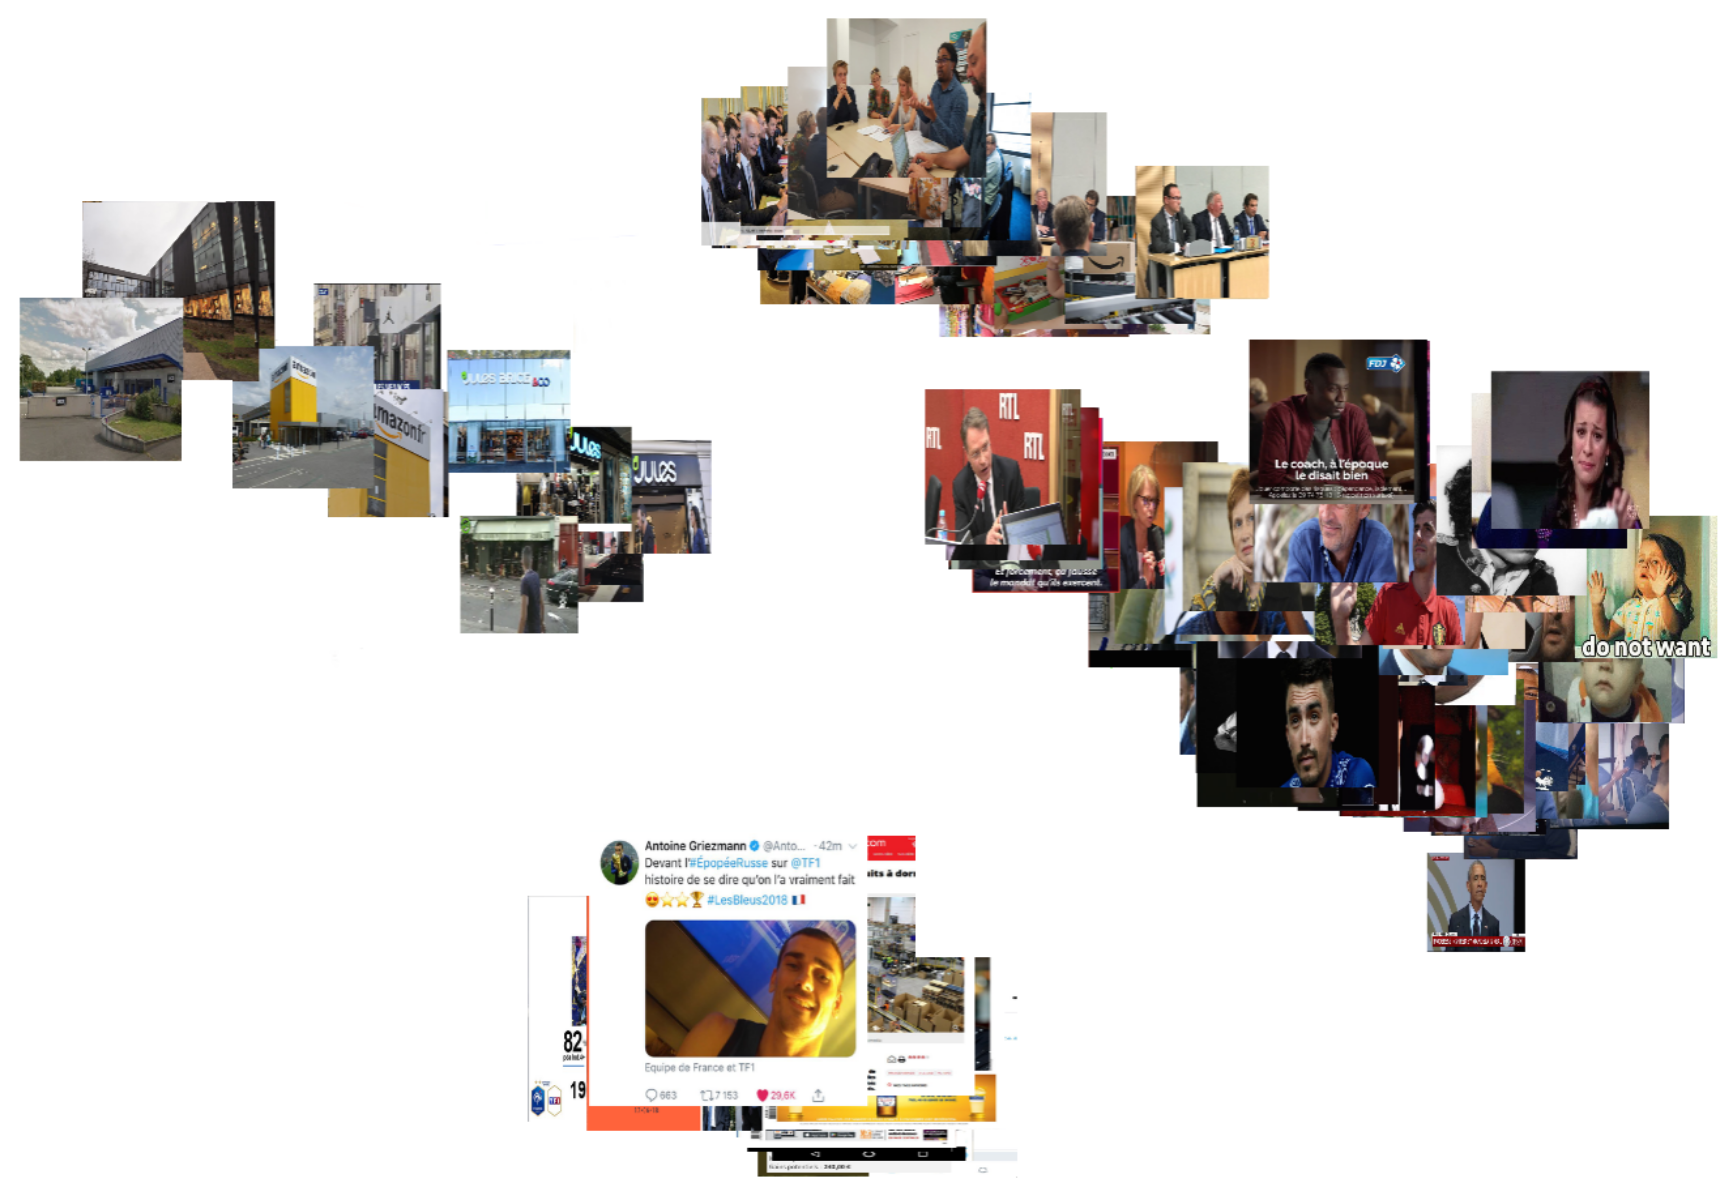
\includegraphics[width=\linewidth]{figures/four_image_clusters.png}
  \caption{Four clusters created using the vizualisation algorithm t-SNE on the ResNet representation of images from our dataset.}
  \label{Fig:t-SNE}
\end{figure}
%%%%%%%%%%%%%%%%%%%%%%%%%%%%%%%%%%%%%%%%%%%%%%%%%%%%%%%%%%%%

In this part we present the different types of embeddings tested for the FSD and re-clustering algorithms. We also report our fine-tuning tests aimed at improving the performance of SBERT on the French corpus. Finally, we detail the text preprocessing applied depending on each model.


\subsection{Types of representations \label{SubSec: representations}}


\subsubsection{Image}

\begin{enumerate}
    \item{\textit{ResNet layer.}} To create image vectors, we test a CNN model trained on ImageNet as the encoder. More precisely, we experiment with the 50 layers version of the ResNet model \citep{he2016deep}. We use the penultimate layer as the vector representation of images. The dimension of the image embedding is $2,048$.
    
    The drawback of this type of representations trained on ImageNet is that the semantic expressed by vectors is categorical: vectors allow distinctions to be made between categories such as "people", "animals", "buildings", but cannot, for example, easily distinguish between two soccer games, or two different buildings. Figure \ref{Fig:t-SNE} illustrates this by showing some of the clusters created using the t-SNE visualization algorithm  \cite{maaten2008visualizing} on images from one day of our dataset represented as ResNet layers. All faces tend to produce similar vectors, whether they are the faces of politicians or "memes" such as the little girl to the right of the picture. On the contrary, the Amazon building is not in the same cluster as the press conference of Amazon executives that appears in one of the pictures above, although a human knowing the company's logo would probably have grouped them together.
    
    \item{\textit{SIFT features.}} Knowing this characteristic of ResNet vectors, we have also used a standard approach based on bag of local features for image descriptions. This category of image retrieval methods is known to integrate low-level visual information, less semantic and more local than that conveyed by global vectors obtained from deep-learning networks. Thus, it focuses on the existence of visually very similar details, in all or part of the images. The underlying idea of this approach is to enable the detection of places or similar objects between images, which can be useful to create links between the tweets. Figure \ref{Fig:Benalla} shows an example of the kind of similarities that can be detected using local features.
    
    All images are described with SIFT features \cite{lowe1999object}, which are then compressed to 128-bit binary hash codes. This is done by first computing a principal component analysis in the original feature space followed by a binary quantization. The distance between any two features can then be efficiently approximated by the Hamming distance between the hash codes. To avoid scanning the whole dataset, the hash codes are then indexed in a hash table whose keys are the $t$-length prefix of the hash codes. At search time, the hash code  of a query feature is computed, as well as its $t$-length prefix. We then use a probabilistic multi-probe search algorithm inspired by the one of \cite{joly2008posteriori} and allowing to efficiently return the approximate K-Nearest Neighbors (K-NN) of each query feature. The raw visual matches returned by the approximate K-NN search are finally filtered by a spatial consistency checking. We therefore estimate a linear transformation (by a RANSAC algorithm) between the query image and each matched image.
    
    We did not use SIFT features to create image vectors, and therefore we cannot test this representation with the FSD algorithm. Moreover, the distance between images is only computed between the query image and its neighbors as returned by the approximate K-NN search algorithm. Therefore, we do not have the complete distance matrix of images and cannot compute an adapted version of the FSD algorithm with a custom distance metric. However, we can use the distance metric between an image and its close neighbours in the second step of our re-clustering method (\ref{SubSec: reclustering}).
    
%%%%%%%%%%%%%%%%%%%%%%%%%%%%%%%%%%%%%%%%%%%%%%%%%%%%%%%%%%%%
\begin{figure}[h]
  \centering
  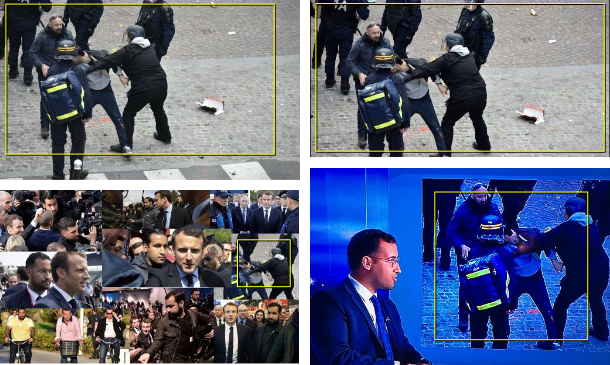
\includegraphics[width=\linewidth]{./figures/Benalla.png}
  \caption{Example of near neighbors detected using SIFT features among the images from our dataset. The first image is used as query, and the following ones are matched neighbors.}
  \label{Fig:Benalla}
\end{figure}
%%%%%%%%%%%%%%%%%%%%%%%%%%%%%%%%%%%%%%%%%%%%%%%%%%%%%%%%%%%%

\end{enumerate}

\subsubsection{Text}
\label{Subsubsec: text}
We chose models having both French and English versions. This sub-section details the models used.

\begin{enumerate}
    \item \textit{Tf-idf.} Due to the inherent brevity of tweets, we simplified the calculation of tf-idf to a simple calculation of idf, since it is rare for a term to be used several times in the same tweet. The form used to calculate the weight of a term $t$ in a tweet is therefore $idf(t) = 1 + log(n+1/df(t)+1)$, where $n$ is the total number of documents in the corpus and $df(t)$ is the number of documents in the corpus that contain $t$.
    
We have distinguished two calculation modes for $n$ and $df(t)$: \textbf{tfidf-dataset} denotes the method that counts only annotated tweets, and \textbf{tfidf-all-tweets} denotes the calculation method that takes into account all tweets in the corpus (38 million tweets) to obtain $n$ and $df(t)$. For each method, we restrict the vocabulary with a list of \textit{stop-words} and a threshold $df_{min}$, the minimum number of tweets that must contain $t$ for it to be included in the vocabulary. In all our experiments, $df_{min}=10$. We thus obtain a vocabulary of nearly 330,000 words in English and 92,000 words in French for \textbf{tfidf-all-tweets}, and 5,000 words in English and 9,000 words in French for \textbf{tfidf-dataset}.

\item \textit{Word2Vec.} We used pre-trained models for English, and trained our own French models. For each corpus, we distinguish between \textbf{w2v-twitter}, models trained on tweets, and \textbf{w2v-news}, models trained on press articles. For English, w2v-twitter is a pre-trained model published by \citet{godin2015multimedia}\footnote{\url{github.com/loretoparisi/word2vec-twitter}} (400 dimensions) and w2v-news is a model trained on Google News and published by Google\footnote{\url{code.google.com/archive/p/word2vec/}}  (300 dimensions). In French, w2v-twitter was trained with the CBOW algorithm on 370 million tweets collected between 2018 and 2019, and w2v-news was similarly trained on 1.9 million AFP dispatches collected between 2011 and 2019. Both models have 300 dimensions.
As Word2Vec provides word embeddings and not sentence embeddings, the representation of tweets is obtained by averaging the word vectors of each word. Two methods were used for averaging: a simple average, and an idf-weighted average using the \textbf{tfidf-all-tweets} calculation method.

\item \textit{ELMo.} For English, we used the model published on TensorFlow Hub\footnote{\url{tfhub.dev/google/elmo/2}}. For French, a model trained on French published by \citet{che2018towards}\footnote{\url{github.com/HIT-SCIR/ELMoForManyLangs}}. In each case, we use the average of the three layers of the network as a representation of each word. The representation of a tweet is produced by averaging these vectors (of dimension $1,024$).


\item \textit{BERT.} Google provides an English model and a multilingual model\footnote{\url{github.com/google-research/bert} models: bert-large, uncased and bert-base, multilingual cased}. In order to improve the performance of the multilingual model on French tweets, we continued training for 150,000 steps on tweets collected in June 2018. We refer to the simple multilingual model as \textbf{bert} and the model trained on tweets as \textbf{bert-tweets}. In each case, we used the penultimate layer of the network (of dimension 768) as embedding, by averaging the tokens to obtain a tweet representation.

\item \textit{Universal Sentence Encoder.}
    \item The provided models\footnote{\url{tfhub.dev/google/universal-sentence-encoder-large/3}}\textsuperscript{,}\footnote{\url{tfhub.dev/google/universal-sentence-encoder-multilingual-large/1}}
    (english and multilingual) are designed to provide sentence embeddings, so we were able to use them as is, without averaging vectors
    like in the previous representations. The vectors are of dimension 512.

\item \textit{Sentence-BERT} The authors of SBERT provide pre-trained models for English\footnote{\url{github.com/UKPLab/sentence-transformers}. Model: bert-large-nli-stsb-mean-tokens}. For French, we had to perform a fine-tuning of the multilingual BERT model, which we present in Section \ref{Subsec: Fine-tuning}. The vectors obtained are of dimension 768.
\end{enumerate}

\subsubsection{Text-image representation}

We build a common vector of text and image by concatenating the ResNet vectors with each type of textual representation. We test several coefficients applied to the image vectors, in order to increase or decrease their weight in the clustering process.


\subsection{Fine-tuning Sentence-BERT for French}
\label{Subsec: Fine-tuning}
%%%%%%%%%%%%%%%%%%%%%%%%%%%%%%%%%%%%%%%%%%%%%%%%%%%%%%%%%%%%
\begin{figure}[h]
  \centering
  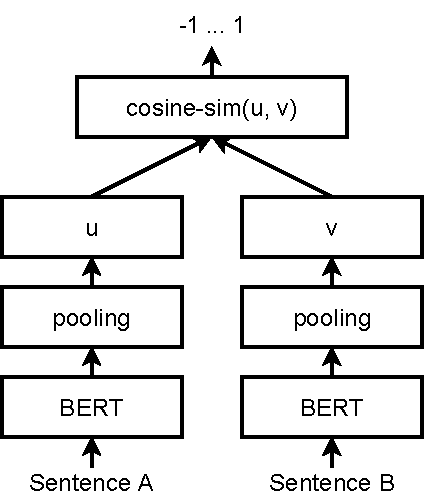
\includegraphics[width=.3\linewidth]{figures/SentenceBERT.pdf}
  \caption{SBERT architecture at inference, to compute similarity scores. This architecture is also used during part of the training with mean-square-error as regression objective function. This diagram is provided in the Sentence-BERT paper \cite{reimers_2019_sentence}.}
  \label{Fig:SBERT}
\end{figure}
%%%%%%%%%%%%%%%%%%%%%%%%%%%%%%%%%%%%%%%%%%%%%%%%%%%%%%%%%%%%
The SBERT model is specifically trained to provide cosine similarity scores: the architecture presented in Figure \ref{Fig:SBERT} is used to train the model
on the STS corpus. The objective function is a mean-square-error loss between $cosine\text{-}sim(u,v)$ and the similarity score evaluated manually in the dataset. This model seems particularly suitable for a clustering algorithm based on cosine similarity, and indeed, among the sentence embeddings (\textit{Universal Sentence Embedding} and SBERT), this it is the one that provides the best clustering results in English.

However, the English pre-trained model is based on fine-tuning on supervised tasks (see \ref{embedding_phrases} for details of SNLI and STS tasks), which cannot be done in French without an annotated corpus. We have therefore implemented two strategies to perform a fine-tuning of the \textbf{bert-tweets} model on French data: first we have used \textit{Cloud Translation API}\footnote{\url{cloud.google.com/translate/docs/reference/rest/}} within the free use limit to translate part of the STS dataset (we obtained $2,984$ pairs of sentences in French). Second, we manually annotated 500 pairs of headlines of selected newspaper articles (we selected headlines that contained common terms). The annotation was done on a scale of 0 to 5, in the same way as for STS. However, instead of indicating the degree of semantic similarity between the sentences, we sought to assess whether the two headlines described the same event. The two types of fine-tuning (translated corpus, or translated corpus + annotated corpus) are designated by \textbf{sbert-tweets-sts-short} and \textbf{sbert-tweets-sts-long}. The performances of the different representations are described in Section \ref{Sec: results}.

\subsection{Preprocessing}

Each text embedding model takes different text formats as inputs: for example, models able to deal with sentences, such as BERT, Sentence-BERT, ELMo or Universal Sentence Encoder, take the full text with punctuation as input. For Word2Vec and tf-idf models, we lowercase characters and remove punctuation. Table \ref{Tab:preprocessing} summarizes all preprocessing steps depending on the type of model. Each column correponds to a preprocessing step:
\begin{itemize}
    \item remove mentions: mentions are a Twitter-specific way of referring to another Twitter user in a tweet, so that she is notified that the tweet is talking about her or is addressed to her. Entries take the following form: @name\_of\_the\_user. For tf-idf models, removing mentions is a way to reduce the size of the vocabulary. For most Word2Vec models, mentions are not part of the vocabulary, except for w2v\_twitter\_en.
    \item unidecode: we use the Python module unidecode to convert Unicode characters to ASCII characters. In French, for example, all accents are removed: "Wikipédia" becomes "Wikipedia".
    \item lower: we set the text in lowercase letters.
    \item hashtag split: we split hashtags on capital letters. "\#HappyEaster" becomes "Happy Easter". This step is of course applied before lowercasing.
    \item remove long numbers: we remove numbers longer than 4 digits.
    \item remove repeated characters: we limit the number of repeated characters inside a word to three. "looooool" becomes "loool".
\end{itemize}

%%%%%%%%%%%%%%%%%%%%%%%%%%%%
\begin{table}
\begin{center}
\resizebox{\textwidth}{!}{%
\rowcolors{2}{white}{gray!25}
\begin{tabular}{lccccccccc}
\hline
                  model & rm mentions & unidecode & lower & rm punctuation & rm stop-words & hashtag split & rm long numbers & rm repeated chars & rm urls \\
\hline
       tfidf\_all\_tweets &           X &         X &     X &              X &             X &             X &               X &                 X &       X \\
          tfidf\_dataset &           X &         X &     X &              X &             X &             X &               X &                 X &       X \\
             w2v\_afp\_fr &           X &         X &     X &              X &               &             X &               X &                 X &       X \\
         w2v\_twitter\_fr &           X &         X &     X &              X &               &             X &               X &                 X &       X \\
           w2v\_gnews\_en &           X &           &       &              X &               &             X &               X &                 X &       X \\
         w2v\_twitter\_en &             &           &       &              X &               &             X &               X &                 X &       X \\
                   elmo &             &           &       &                &               &             X &               X &                 X &       X \\
                   bert &             &           &       &                &               &             X &               X &                 X &       X \\
            bert\_tweets &             &           &       &                &               &             X &               X &                 X &       X \\
              sbert\_sts &             &           &       &                &               &             X &               X &                 X &       X \\
          sbert\_nli\_sts &             &           &       &                &               &             X &               X &                 X &       X \\
 sbert\_tweets\_sts\_short &             &           &       &                &               &             X &               X &                 X &       X \\
  sbert\_tweets\_sts\_long &             &           &       &                &               &             X &               X &                 X &       X \\
                    use &             &           &       &                &               &             X &               X &                 X &       X \\
\hline
\end{tabular}

}
\end{center}
\caption{Preprocessing applied for each model \label{Tab:preprocessing}}
\end{table}
%%%%%%%%%%%%%%%%%%%%%%%%%%%%

\section{Results}
\label{Sec: results}

\subsection{Comparison of text embeddings}
\label{Subsec: text embeddings}
Whether for the classification task or for the clustering task, none of the tested models manage to outperform the tf-idf model calculated on the whole corpus (tfidf-all-tweets). However, the relative performance of the models varies by language, and by task. 

SVM classification results are consistent and robust to kernel change (see Tables \ref{classif_en} and \ref{classif_fr}). They show that BERT and ELMo do not provide easily separable short-text vectors. Models intended to be used as embeddings (Word2Vec, \textit{Universal Sentence Encoder}, SBERT) obtain better results. On the French corpus, the results of these models are similar to those of tf-idf vectors. On the English corpus, the tf-idf vectors remain the best adapted,  on a par with weighted w2v-news vectors. 

%%%%%%%%%%%%%%%%%%%%%%%%%%%%
\begin{table}[ht]
\begin{center}
\rowcolors{2}{gray!25}{white}
\begin{tabular}{|l|ccc|cccc|}
\hline
                           &\multicolumn{3}{c}{\textbf{Triangular Kernel}}&\multicolumn{4}{|c|}{\textbf{RBF Kernel}}\\
\cline{2-8}    \textbf{Model} &       \textit{F1} &        \textit{p} &        \textit{r} & $\gamma$ &       \textit{F1} &        \textit{p} &        \textit{r} \\
\hline
             bert  &  74.49 $\pm$ 0.41 &  85.76 $\pm$ 0.56 &  69.42 $\pm$ 0.38 &     0.01 &  75.31 $\pm$ 0.51 &  85.10 $\pm$ 0.62 &  70.87 $\pm$ 0.52 \\
             elmo  &  59.81 $\pm$ 0.41 &  77.17 $\pm$ 0.63 &  53.23 $\pm$ 0.25 &     0.10 &  57.64 $\pm$ 0.36 &  77.18 $\pm$ 0.29 &  50.55 $\pm$ 0.28 \\
    sbert-nli-sts  &  80.55 $\pm$ 0.33 &  87.85 $\pm$ 0.35 &  76.94 $\pm$ 0.31 &     0.01 &  80.37 $\pm$ 0.36 &  88.53 $\pm$ 0.37 &  76.26 $\pm$ 0.32 \\
 tfidf-all-tweets  &\textbf{83.50} $\pm$ 0.78 &  90.87 $\pm$ 0.47 &  79.91 $\pm$ 0.78 &     1.00 &\textbf{81.86} $\pm$ 0.77 &  90.98 $\pm$ 0.32 &  77.41 $\pm$ 0.79 \\
    tfidf-dataset  &\textbf{83.46} $\pm$ 0.72 &  90.28 $\pm$ 0.51 &  80.08 $\pm$ 0.71 &     1.00 &\textbf{82.70} $\pm$ 0.69 &  89.67 $\pm$ 0.51 &  79.10 $\pm$ 0.73 \\
              use  &  80.26 $\pm$ 0.38 &  86.17 $\pm$ 0.29 &  77.59 $\pm$ 0.40 &     1.00 &  79.92 $\pm$ 0.46 & 85.68 $\pm$ 0.45 &  77.40 $\pm$ 0.40 \\
         w2v-news  &  81.35 $\pm$ 0.53 &  88.94 $\pm$ 0.40 &  77.45 $\pm$ 0.65 &     1.00 &  80.42 $\pm$ 0.55 & 89.09 $\pm$ 0.41 &  75.89 $\pm$ 0.64 \\
    w2v-news tfidf &\textbf{82.39} $\pm$ 0.64 &  89.00 $\pm$ 0.35 &  79.02 $\pm$ 0.69 &     0.01 &\textbf{81.57} $\pm$ 0.73 &  89.02 $\pm$ 0.51 &  77.64 $\pm$ 0.78 \\
      w2v-twitter  &  76.68 $\pm$ 0.53 &  86.82 $\pm$ 0.53 &  72.24 $\pm$ 0.52 &     10.0 &  77.62 $\pm$ 0.62 &  87.91 $\pm$ 0.39 &  72.71 $\pm$ 0.68 \\
 w2v-twitter tfidf &  81.20 $\pm$ 0.48 &  88.67 $\pm$ 0.17 &  77.54 $\pm$ 0.54 &     0.10 &  81.07 $\pm$ 0.49 &  88.61 $\pm$ 0.29 &  77.24 $\pm$ 0.59 \\
\hline
\end{tabular}

\\

{\scriptsize \textbf{Note:} Each cell indicates the mean and standard deviation of 5 runs (with different train/test splits), in percentages.}
\caption{SVM classification results on the English corpus} \label{classif_en}
\end{center}
\end{table}
%%%%%%%%%%%%%%%%%%%%%%%%%%%%

%%%%%%%%%%%%%%%%%%%%%%%%%%%%
\begin{table}[ht]
\begin{center}
\rowcolors{2}{gray!25}{white}
\begin{tabular}{|l|ccc|cccc|}
\hline
                           &\multicolumn{3}{c}{\textbf{Triangular Kernel}}&\multicolumn{4}{|c|}{\textbf{RBF Kernel}}\\
\cline{2-8}
    \textbf{Model} &       \textit{F1} &        \textit{p} &        \textit{r} & $\gamma$ &      \textit{F1} &        \textit{p} &        \textit{r} \\
\hline
             bert  &  78.46 $\pm$ 0.68 &  90.88 $\pm$ 0.78 &   71.26 $\pm$ 0.7 &        - &                - &                 - &                 - \\
      bert-tweets  &   81.77 $\pm$ 0.7 &  91.88 $\pm$ 0.95 &  75.73 $\pm$ 0.75 &      0.1 &  57.12 $\pm$ 0.2 &  90.44 $\pm$ 0.55 &  45.11 $\pm$ 0.11 \\
             elmo  &  73.59 $\pm$ 0.64 &  88.53 $\pm$ 0.74 &  65.54 $\pm$ 0.61 &        - &                - &                 - &                 - \\
   sbert-tw-sts-l  &  86.08 $\pm$ 0.86 &   93.6 $\pm$ 0.94 &  81.16 $\pm$ 0.81 &        - &                - &                 - &                 - \\
 tfidf-all-tweets  &  87.79 $\pm$ 0.58 &  95.24 $\pm$ 0.91 &   83.13 $\pm$ 0.5 &        - &                - &                 - &                 - \\
    tfidf-dataset  &  87.66 $\pm$ 0.69 &  94.78 $\pm$ 1.15 &  83.14 $\pm$ 0.53 &        - &                - &                 - &                 - \\
              use  &   87.45 $\pm$ 0.6 &  93.94 $\pm$ 0.56 &  83.44 $\pm$ 0.58 &        - &                - &                 - &                 - \\
         w2v-news  &   86.59 $\pm$ 0.8 &  92.82 $\pm$ 1.03 &  82.63 $\pm$ 0.74 &        - &                - &                 - &                 - \\
    w2v-news tfidf &  87.51 $\pm$ 0.71 &  92.94 $\pm$ 1.06 &  84.02 $\pm$ 0.49 &        - &                - &                 - &                 - \\
      w2v-twitter  &  87.01 $\pm$ 0.56 &   93.4 $\pm$ 0.84 &  83.03 $\pm$ 0.58 &        - &                - &                 - &                 - \\
 w2v-twitter tfidf &  87.73 $\pm$ 0.56 &  93.51 $\pm$ 0.99 &  84.03 $\pm$ 0.38 &        - &                - &                 - &                 - \\
\hline
\end{tabular}

\\

{\scriptsize \textbf{Note:} Each cell indicates the mean and standard deviation of 5 runs (with different train/test splits), in percentages.}
\caption{SVM classification results on the French corpus} \label{classif_fr}
\end{center}
\end{table}
%%%%%%%%%%%%%%%%%%%%%%%%%%%%

%%%%%%%%%%%%%%%%%%%%%%%%%%%%
\begin{table}[ht]
\begin{center}
\rowcolors{2}{gray!25}{white}
\begin{tabular}{|l|cc|cc|}
\hline
\rowcolor{gray!25}                           &\multicolumn{2}{c}{\textbf{English}}&\multicolumn{2}{|c|}{\textbf{French}}\\
\cline{2-5}
                   \textbf{Model}  & \textit{t} & \textit{F1} & \textit{t} & \textit{F1} \\
\hline
                     bert  &       0.04 &       39.22 &       0.04 &       44.79 \\
              bert-tweets  &          - &           - &       0.02 &       50.02 \\
                     elmo  &       0.08 &       22.48 &       0.20 &       46.08 \\
            sbert-nli-sts  &       0.39 &       58.24 &          - &           - \\
    sbert-tweets-sts-long  &          - &           - &       0.36 &       67.89 \\
   sbert-tweets-sts-short  &          - &           - &       0.38 &       65.71 \\
         tfidf-all-tweets  &       0.75 &\textbf{70.10}&      0.70 &\textbf{78.05}\\
            tfidf-dataset  &       0.65 &       68.07 &       0.70 &       74.39 \\
                      use  &       0.22 &       55.71 &       0.46 &       74.57 \\
                 w2v-news  &       0.30 &       53.99 &       0.25 &       66.34 \\
    w2v-news tfidf-weights &       0.31 &       61.81 &       0.30 &       75.55 \\
              w2v-twitter  &       0.16 &       43.20 &       0.15 &       57.53 \\
 w2v-twitter tfidf-weights &       0.20 &       53.45 &       0.25 &       71.73 \\
\hline
\end{tabular}

\\

{\scriptsize \textbf{Note:} Performance is assessed using the "Best Matching F1" score.\\ 
For each model, the best $t$ threshold value was selected by successive tests.}
\caption{FSD clustering results for each corpus} \label{clustering}
\end{center}
\end{table}
%%%%%%%%%%%%%%%%%%%%%%%%%%%%

The tfidf-all-tweets vectors also give the best results for the clustering task (see Table \ref{clustering}), even more clearly than for classification. This is due to the shape of the tf-idf vectors, which are particularly well suited for cosine similarity calculations, as well as to the event-specific characteristics of the two datasets: the same terms are obviously widely used among tweets of the same event.
These results are consistent with those of \citet{cage2020production}, who came to similar conclusions regarding event detection in press articles.

Concerning neural models adapted to sentence embeddings (SBERT, \textit{Universal Sentence Encoder}), they do not perform better than the tf-idf weighted w2v-news models. On the English corpus, we note that the fine-tuning of \textit{Sentence-BERT} on semantic similarity corpora (sbert-nli-sts) allows slightly better results than the generic vectors of \textit{Universal Sentence Encoder}.

Our own fine-tuning of BERT (sbert-tweets-sts-short and sbert-tweets-sts-long) does not outperform \textit{Universal Sentence Encoder} on the French corpus. However, we note that the thematic similarity corpus (which contains only 500 pairs of sentences) allows to increase the clustering performance by 2 points. Nevertheless, our fine-tuning does not achieve as good results as the English model, due to the fact that it could not be trained on a corpus of similar size to SNLI.

When used with the FSD algorithm, the 
best embeddings (tf-idf, Word2Vec with tf-idf weights,
Universal Sentence Encoder) also have the property to be
less sensitive to variations of the threshold $t$, as shown in
Figure \ref{fig: graph_FSD}. Moreover, the optimal value of $t$ for a
given embedding seems to be approximately the same for
each corpus (0.7 for tf-idf). This result may indicate that
the First Story Detection algorithm could be applied to
other (not annotated) tweet datasets without adapting the
threshold value.

%%%%%%%%%%%%%%%%%%%%%%%%%%%%%%%%%%%%%%%%%%%%%%%%%%%%%%%%%%%%%%%
\begin{figure}
\centering
\begin{subfigure}{.5\textwidth}
  \centering
  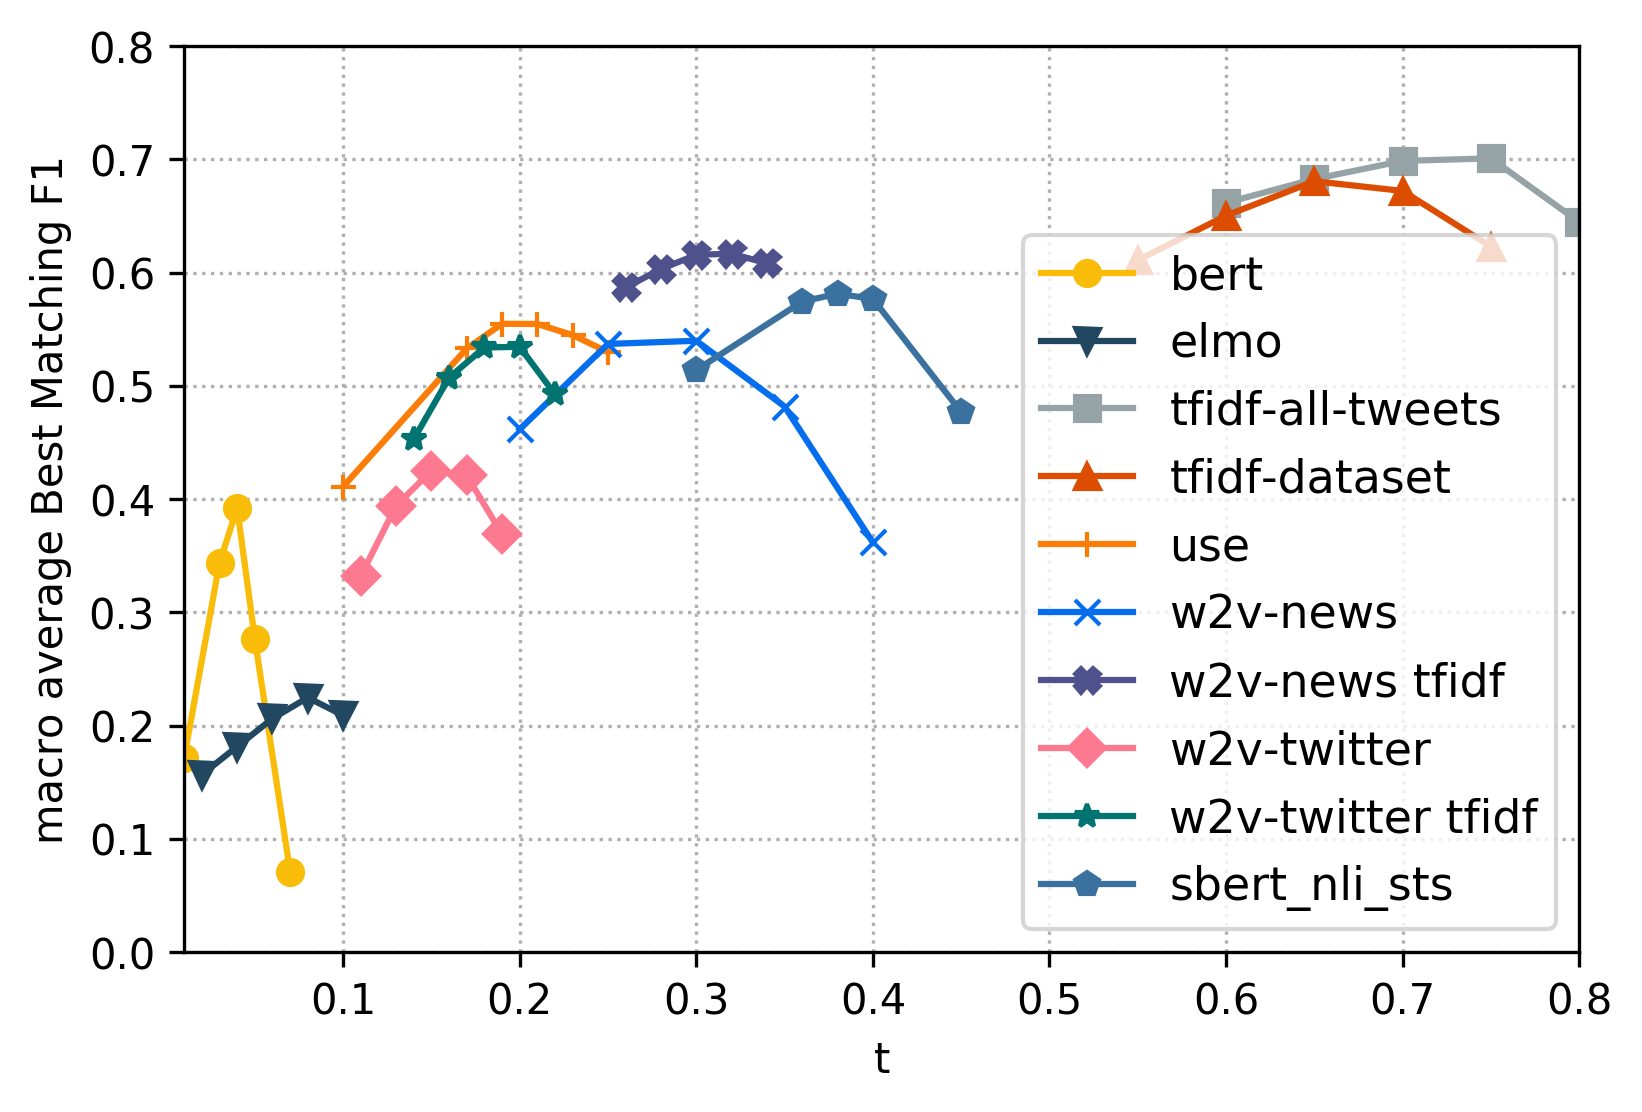
\includegraphics[width=1\linewidth]{figures/graph_en_FSD.png}
  \caption{English}
  \label{fig: graph_FSD_en}
\end{subfigure}%
\begin{subfigure}{.5\textwidth}
  \centering
  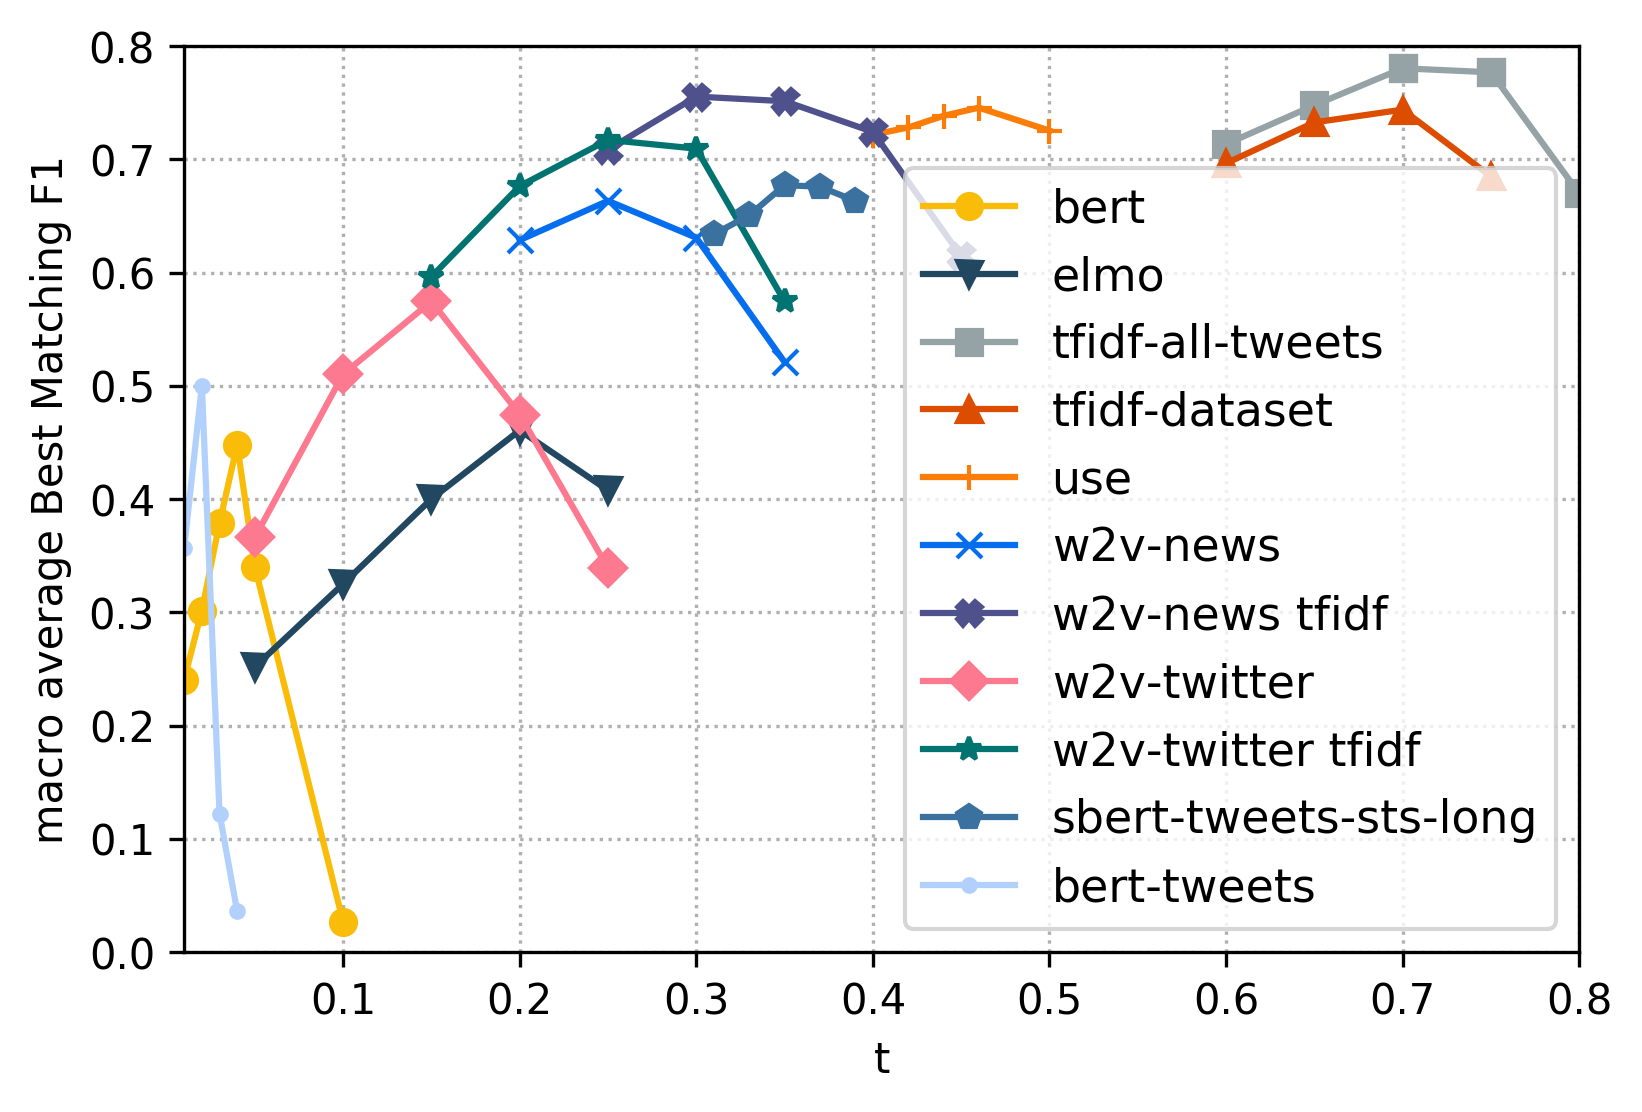
\includegraphics[width=1\linewidth]{figures/graph_fr_FSD.png}
  \caption{French}
  \label{fig: graph_FSD_fr}
\end{subfigure}
\caption{Best Matching F1 score for FSD clustering depending on the
threshold parameter $t$ for each corpus}
\label{fig: graph_FSD}
\end{figure}
%%%%%%%%%%%%%%%%%%%%%%%%%%%%%%%%%%%%%%%%%%%%%%%%%%%%%%%%%%%%%%

It is surprising that Word2Vec models trained on tweets are no better than models trained on news. However, this can be explained by two factors: the content of the datasets, which are made up of tweets referring to news, and whose vocabulary is therefore probably closer to the corpus from the AFP or from Google News than to the average Twitter. The second factor is the great variability in the vocabulary of tweets: it is possible that the w2v\_twitter\_en model, trained on tweets from 2015, does not correspond to the vocabulary used in the \citet{mcminn_building_2013} corpus, collected in 2012.

The better performance on the French corpus than on the English corpus is probably due to the fact that classification
and clustering on the English corpus are more difficult tasks, for several reasons: first, the English corpus is from
2012, and therefore an important part of the tweets have been deleted (our last download in November 2019 allowed us to
retrieve 72,484 tweets \textit{i.e.} 72\% of the original annotated dataset). This can have important consequences,
especially for the FSD algorithm which over-segments clusters if a tweet is missing to link them.
Second, it seems that many events in the English corpus could be considered as
"sub-events" of the same macro event:
"Hurricane Sandy in the Bahamas", "Tweets for Praying for people affected by the hurricane sandy", "Superstorm Sandy
hits the east coast of the USA.", "They all discuss about Sandy Storm" are for example four different events in the
corpus by \citet{mcminn_building_2013}. These events with very close topical similarity are probably more difficult to
separate for the algorithm.

\subsection{Comparison of text-image embeddings}
\label{Subsec: text-image embeddings}
%%%%%%%%%%%%%%%%%%%%%%%%%%%%
\begin{table}[ht]
\begin{center}
\rowcolors{2}{white}{gray!25}
\begin{tabular}{|l|ccccc|}
\hline
             \textbf{Model} &   $t$ &  \textit{F1} &  \textit{precision} &  \textit{recall} & \textit{weight} \\
\hline
                       elmo &  0.23 &         50.1 &                77.5 &             50.1 &                 \\
              elmo / resnet &  0.28 &         52.5 &                80.2 &             50.3 &            0.05 \\
           tfidf-all-tweets &  0.79 &         84.3 &                92.5 &             83.7 &                 \\
  tfidf-all-tweets / resnet &  0.79 &         84.6 &                92.3 &             84.3 &           0.005 \\
                   w2v-news &  0.28 &         75.5 &                88.1 &             74.8 &                 \\
          w2v-news / resnet &  0.35 &         76.9 &                87.2 &             77.9 &            0.01 \\
             w2v-news tfidf &  0.40 &         81.7 &                89.1 &             83.4 &                 \\
    w2v-news tfidf / resnet &  0.39 &         82.1 &                90.6 &             82.3 &            0.01 \\
                w2v-twitter &  0.17 &         66.5 &                85.2 &             66.0 &                 \\
       w2v-twitter / resnet &  0.20 &         69.2 &                87.5 &             66.8 &            0.01 \\
          w2v-twitter tfidf &  0.29 &         79.0 &                90.4 &             78.9 &                 \\
 w2v-twitter tfidf / resnet &  0.29 &         79.0 &                90.4 &             79.0 &           0.005 \\
\hline
\end{tabular}

\\

{\scriptsize \textbf{Note:} Performance is assessed using the "Best Matching F1" score.\\ 
For each model, the best $t$ threshold value was selected by successive tests.}
\caption{FSD clustering results on "text only" and "text-image" vectors on the tweets of the French corpus that include visual content} \label{Tab: text_image}
\end{center}
\end{table}
%%%%%%%%%%%%%%%%%%%%%%%%%%%%
The results presented in this section concern only our dataset, as the English dataset does not include enough images: among the annotated tweets that we were able to retrieve, only 570 contained a link to a video, image or animated GIF. In 2012, the use of smartphones was much more restricted than at present, which probably explains the small number of images.

Conversely, our dataset built up in 2018 contains many visual contents. Among the 95,796 annotated tweets, we were able to download multimedia content for 22,477 of them (19.8\% photos, 2.5\% videos and 1.5\% GIFs). In order to get the highest possible number of images, we processed videos and GIFs as images by using the thumbnails provided by Twitter for a static display.  We thus obtained 20,481 unique images. We only considered tweets containing visual contents for clustering, which is why the clustering results that we present below are slightly different from those of the previous part, even for the text-only methods.


%%%%%%%%%%%%%%%%%%%%%%%%%%%%%%%%%%%%%%%%%%%%%%%%%%%%%%%%%%%%
\begin{figure}[h]
  \centering
  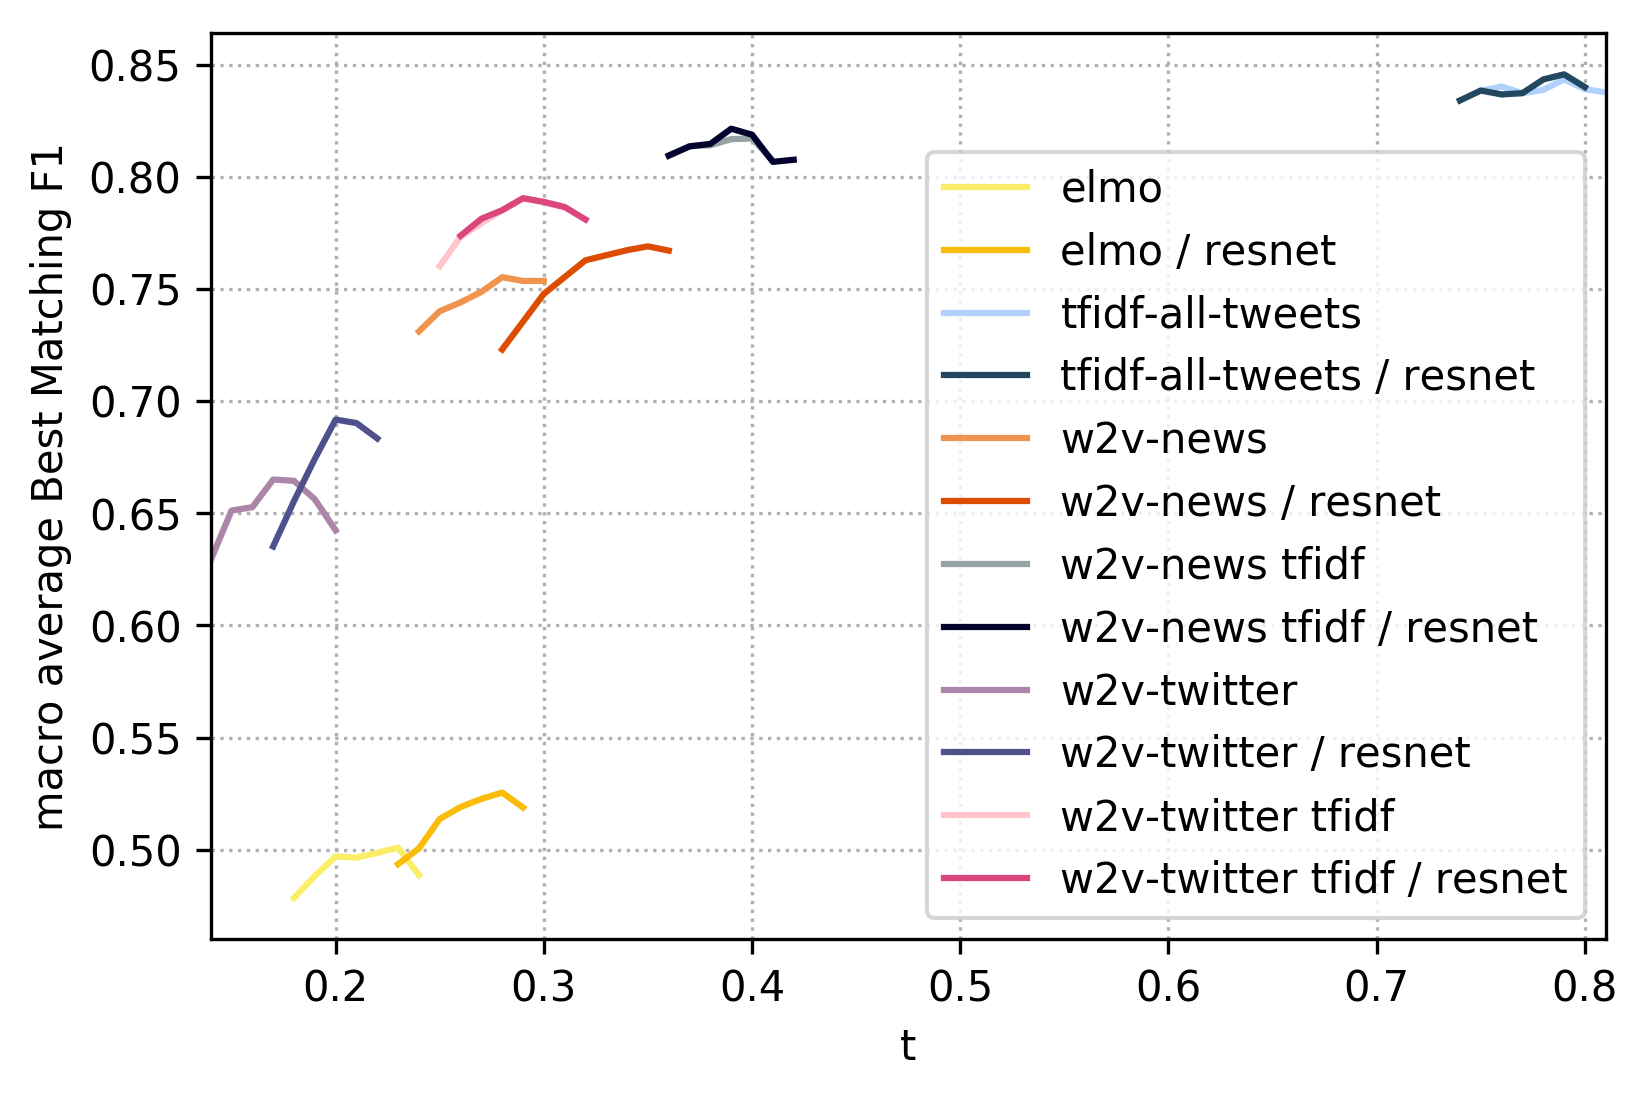
\includegraphics[width=.7\linewidth]{figures/text_image_clustering.png}
  \caption{Best Matching F1 score for FSD clustering depending on the treshold parameter $t$ for text-only and text-image vectors on the tweets of the French corpus that include visual content}
  \label{Fig:text-image}
\end{figure}
%%%%%%%%%%%%%%%%%%%%%%%%%%%%%%%%%%%%%%%%%%%%%%%%%%%%%%%%%%%%


We present the clustering results in Table \ref{Tab: text_image}. These results show that visual features do not bring a significant gain a performance to the FSD algorithm. Image may improve the results of the textual representations that perform the worst (ELMo). However, this gain is not significant enough to outperform the tf-idf representation. Moreover, the weights applied to the ResNet layer before it is concatenated with textual features are extremely small (0.005 for the tf-idf / ResNet concatenation). This in an indication of the very small role played by visual features in the nearest neighbor search. Figure \ref{Fig:text-image} illustrates this result more clearly by showing the change in macro-F1 depending on $t$: ELMo and Word2Vec embeddings are distinctly improved through the concatenation with visual features, whereas the tf-idf embedding provides the same results when it is combined with the ResNet layer.

\subsection{Comparison of event detection methods}

In the previous parts (\ref{Subsec: text embeddings} and \ref{Subsec: text-image embeddings})  we have determined the best embeddings to serve as input to the FSD algorithm. We now compare our best results with those obtained with other methods: re-clustering, DBSCAN and DMM.

%%%%%%%%%%%%%%%%%%%%%%%%%%%%
\begin{table}[ht]
\begin{center}
\begin{tabular}{|l|cccccc|}
\hline
  \textbf{Algorithm} &   $t$ & $t_1$ & $p_1$ &  \textit{F1} &  \textit{precision} &  \textit{recall} \\
\hline
      FSD with tfidf &  0.79 &     - &     - &         84.3 &                92.5 &             83.7 \\
 reclustering ResNet &  0.60 &     5 &   0.8 &         79.6 &                91.9 &             77.3 \\
   reclustering SIFT &  0.60 &   -24 &   0.9 &         81.1 &                96.7 &             74.3 \\
\hline
\end{tabular}

\\

{\scriptsize \textbf{Note:} Performance is assessed using the "Best Matching F1" score.\\ 
For each model, the best $t$, $t_1$ and $p_1$ values were selected by successive tests.}
\caption{Clustering performance of the FSD algorithm and re-clustering algorithms on the tweets of the French corpus that include visual content} \label{Tab: reclustering}
\end{center}
\end{table}
%%%%%%%%%%%%%%%%%%%%%%%%%%%%
Table \ref{Tab: reclustering} shows the results of the re-clustering approach using each type of visual representation: either a semantic representation, with ResNet vectors, or local features representation, with SIFT similarities. These results indicate that local features tend to perform best to improve the first clustering step. Overall, however, this way of combining representations degrades the performance of the FSD algorithm alone. The very high values selected for the $p_1$ parameter, that indicate that very few clusters are allowed to merge, seem to indicate that the only way to obtain correct results with the re-clustering algorithm is to minimize the role of the second step. The obtained results are thus close to the results of the FSD algorithm alone with a too low $t$ parameter.

The comparative results of DBSCAN, DMM and FSD are summarized in Table \ref{}. The First Story Detection algorithm outperforms the other tested methods by a clear margin on both datasets.

\subsection{Results on the entire collection}
All previous experiments were conducted on the annotated part of our dataset. However, the final objective of our study is to detect events in the entire collection of tweets (4.5 million tweets per day on average) and over a period of several months. In order to be able to process such a large amount of tweets in an acceptable time frame, we had to introduce some modifications to the "Mini Batch FSD" algorithm presented in Section \ref{Subsec: FSD}. These changes also aim to manage the large volume of "noise" (very short documents, whose subject is difficult to know, even for a human reader) naturally present in a dataset of non-pre-selected tweets.

The changes are as follows: 
\begin{itemize}
    \item a tweet is considered irrelevant if its tf-idf vector does not contain any element with a value greater than a $r$ threshold. In other words, the tweet contains only extremely common words;
    \item  a tweet is also considered irrelevant if it contains less than $m$ words. 
\end{itemize}
Irrelevant tweets can be clustered if a nearest neighbor is found, however, if no nearest neighbor is found within a radius $t$ they are excluded from the collection and labelled as $-2$. Whether they are clustered or not, irrelevant tweets cannot be selected as nearest neighbors in the following iterations of the algorithm. 

This method has two advantages: first, it prevents very vague tweets from extending the vocabulary of the cluster to which they are attached. This reinforces the stability of the vocabulary of each cluster. Second, it reduces the number of past tweets to which each tweet must be compared, thus increasing the time efficiency of the algorithm. Indeed, the complexity of the FSD algorithms shifts from $O(nw)$ (with $n$ the number of documents in the collection and $w$ the number of documents in the comparison window) to $O(nwp)$, with $p$ the proportion of relevant tweets in the collection.

We tested this improvement on the entire corpus (retweets excluded), i.e. 38 million tweets, with the following parameters: $t=0.6, r=0.21, m=5$. The value of $r$ was calculated from our annotated dataset as follows: 
\begin{align*}
r = \min_{d \in C}\max_{w \in d}idf(w)
\end{align*}
Thus, we select the minimum value of $r$ on a dataset where all tweets are considered relevant. Any tweet from the rest of the collection that has no word of at least this significance is considered irrelevant. The results of both methods (with and without relevance thresholds) are displayed in Table \ref{Tab: FSD_thresholds}. The method with relevance thresholds seems to obtain better scores, but these results must be interpreted with caution: indeed, the thresholds "fit" the algorithm to the characteristics of the annotated corpus, resulting in better performance on annotated tweets. This does not tell us whether performance is also better over the entire collection. However, it can legitimately be assumed that these rather low thresholds do not degrade performance, while allowing a gain in time efficiency.

%%%%%%%%%%%%%%%%%%%%%%%%%%%%
\begin{table}[ht]
\begin{center}
\begin{tabular}{|l|cccccc|}
\hline
               \textbf{Algorithm} &  $t$ &  $m$ &   $r$ &  \textit{F1} &  \textit{precision} &  \textit{recall} \\
\hline
 FSD without relevance thresholds &  0.6 &    0 &  0.00 &        52.68 &               74.51 &            52.63 \\
    FSD with relevance thresholds &  0.6 &    5 &  0.21 &        59.82 &               85.07 &            53.68 \\
\hline
\end{tabular}

\\

{\scriptsize \textbf{Note:} Performance is assessed using the "Best Matching F1" score on the annotated tweets of the collection.}
\caption{Clustering performance of the FSD algorithm with and without relevance thresholds} \label{Tab: FSD_thresholds}
\end{center}
\end{table}
%%%%%%%%%%%%%%%%%%%%%%%%%%%%


\section{Conclusion}

This chapter does not provide any new algorithm, only some improvements of the "First Story Detection" algorithm. However, it allows us to verify, on two tweets corpora, some results already established on news corpora \cite{cage2020production}. First, we show that the FSD algorithm is extremely efficient for tweets clustering, more than topic modeling techniques such as Dirichlet Multinomial Mixture model \cite{yin_dirichlet_2014}, or a standard algorithm such as DBSCAN \cite{ester1996density}.  The reason for this superiority probably comes from the very rapid evolution over time of the vocabulary used to talk about a given event. The two previously mentioned algorithms are not designed to take this temporal evolution into account, unlike the FSD algorithm, which allows a gradual evolution of clusters over time.

Second, we show, among a large panel of embedding methods, that the tf-idf weighting remains the most suitable representation of documents for an algorithm such as FSD, that is based on nearest neighbor search with cosine similarity. In addition, tf-idf is not only the representation that provides the best results, but also the most stable to changes in the algorithm parameter (threshold $t$). These are important results for us, and I think for many researchers who are looking to use vector representations of short texts for Information Retrieval tasks. This does not mean that recent neural embedding methods will not eventually outperform tf-idf for this kind of tasks as well. In fact, we would like in future work to re-test BERT's fine-tuning (bert-tweets) with a model specially trained on French like CamemBERT \cite{martin2020camembert} and not a multimodal model. We would also like to test fine-tuning of Sentence-BERT on a forthcoming French corpus of semantic similarity \cite{cardon2020french}, and further explore the idea that semantic similarity (two sentences mean the same thing) and thematic similarity (two sentences talk about the same subject) are two different things that require different approaches.

Finally, we provide partial results on the role of image for the clustering of tweets. It is true that our two approaches to include multimodality (vector concatenation and re-clustering) in clustering are quite naive and could be improved with a more appropriate text-image fusion method. However this is a first step, which suggests that image in tweets is more often a source of additional noise than a source of additional information.



